%%%%%%%%%%%%%%%%%%%%%%%%%%%%%%%%%%%%%%%%%%%%%%%%%%%%%%%%%%%%%%%%%%%%%%%%%%%%
% AGUJournalTemplate.tex: this template file is for articles formatted with LaTeX
%
% This file includes commands and instructions
% given in the order necessary to produce a final output that will
% satisfy AGU requirements, including customized APA reference formatting.
%
% You may copy this file and give it your
% article name, and enter your text.
%
% guidelines and troubleshooting are here: 

%% user added for convenience, can be removed before submission:



%% To submit your paper:
\documentclass[draft]{agujournal2019}
\usepackage{url} %this package should fix any errors with URLs in refs.
\usepackage{lineno}
\usepackage[inline]{trackchanges} %for better track changes. finalnew option will compile document with changes incorporated.
\usepackage{soul}

% MY OWN ADDED PACKAGES TO RENDER UNITS
\usepackage{gensymb}
\usepackage{booktabs}
\usepackage{siunitx}

\linenumbers
%%%%%%%
% As of 2018 we recommend use of the TrackChanges package to mark revisions.
% The trackchanges package adds five new LaTeX commands:
%
%  \note[editor]{The note}
%  \annote[editor]{Text to annotate}{The note}
%  \add[editor]{Text to add}
%  \remove[editor]{Text to remove}
%  \change[editor]{Text to remove}{Text to add}
%
% complete documentation is here: http://trackchanges.sourceforge.net/
%%%%%%%

\draftfalse

%% Enter journal name below.
%% Choose from this list of Journals:
%
% JGR: Atmospheres
% JGR: Biogeosciences
% JGR: Earth Surface
% JGR: Oceans
% JGR: Planets
% JGR: Solid Earth
% JGR: Space Physics
% Global Biogeochemical Cycles
% Geophysical Research Letters
% Paleoceanography and Paleoclimatology
% Radio Science
% Reviews of Geophysics
% Tectonics
% Space Weather
% Water Resources Research
% Geochemistry, Geophysics, Geosystems
% Journal of Advances in Modeling Earth Systems (JAMES)
% Earth's Future
% Earth and Space Science
% Geohealth
%
% ie, \journalname{Water Resources Research}

\journalname{Enter journal name here}


\begin{document}

%%%%%%%%%%%%%%%%%%%%%%%%%%%%%%%%%%%%%%%%%%%%%%%
%  TITLE
%
% (A title should be specific, informative, and brief. Use
% abbreviations only if they are defined in the abstract. Titles that
% start with general keywords then specific terms are optimized in
% searches)
%
%%%%%%%%%%%%%%%%%%%%%%%%%%%%%%%%%%%%%%%%%%%%%%%

% Example: \title{This is a test title}

\title{Climate-driven phytoplankton community variability in the Cariaco Basin, Venezuela}

%%%%%%%%%%%%%%%%%%%%%%%%%%%%%%%%%%%%%%%%%%%%%%%
%
%  AUTHORS AND AFFILIATIONS
%
%%%%%%%%%%%%%%%%%%%%%%%%%%%%%%%%%%%%%%%%%%%%%%%

% Authors are individuals who have significantly contributed to the
% research and preparation of the article. Group authors are allowed, if
% each author in the group is separately identified in an appendix.)

% List authors by first name or initial followed by last name and
% separated by commas. Use \affil{} to number affiliations, and
% \thanks{} for author notes.
% Additional author notes should be indicated with \thanks{} (for
% example, for current addresses).

% Example: \authors{A. B. Author\affil{1}\thanks{Current address, Antartica}, B. C. Author\affil{2,3}, and D. E.
% Author\affil{3,4}\thanks{Also funded by Monsanto.}}

\authors{Benjamin Post\affil{1,2}, Esteban Acevedo-Trejos\affil{3}, Subhendu Chakraborty\affil{1}, Andrew D. Barton\affil{4}, Agostino Merico\affil{1}}


% \affiliation{1}{First Affiliation}
% \affiliation{2}{Second Affiliation}
% \affiliation{3}{Third Affiliation}
% \affiliation{4}{Fourth Affiliation}

\affiliation{1}{Systems Ecology Group, Leibniz Centre for Tropical Marine Research (ZMT), Bremen, Germany}
\affiliation{2}{School of Science, Constructor University, Bremen, Germany}
\affiliation{3}{Earth Surface Process Modelling, GFZ German Research Centre for Geosciences, Potsdam, Germany}
\affiliation{4}{Scripps Institution of Oceanography and Department of Ecology, Behavior and Evolution, University of California San Diego, La Jolla, CA, United States}
%(repeat as many times as is necessary)


% Corresponding author mailing address and e-mail address:

% (include name and email addresses of the corresponding author.  More
% than one corresponding author is allowed in this LaTeX file and for
% publication; but only one corresponding author is allowed in our
% editorial system.)

% Example: \correspondingauthor{First and Last Name}{email@address.edu}

\correspondingauthor{Benjamin Post}{benjaminpost@aoop.de}



%%%%%%%%%%%%%%%%%%%%%%%%%%%%%%%%%%%%%%%%%%%%%%%
% KEY POINTS
%%%%%%%%%%%%%%%%%%%%%%%%%%%%%%%%%%%%%%%%%%%%%%%
%  List up to three key points (at least one is required)
%  Key Points summarize the main points and conclusions of the article
%  Each must be 140 characters or fewer with no special characters or punctuation and must be complete sentences

% Example:
% \begin{keypoints}
% \item	List up to three key points (at least one is required)
% \item	Key Points summarize the main points and conclusions of the article
% \item	Each must be 140 characters or fewer with no special characters or punctuation and must be complete sentences
% \end{keypoints}

\begin{keypoints}
\item The CARIACO time series showed a highly variable phytoplankton community over the course of sampling between 1995 and 2017. Clustering of community data from microscopy cell counts reveals two separate clusters, defined by high- and low-upwelling conditions that match the anomalies in the AMO index. 
% \index Previous studies proposed a shift in the community, but with the full dataset we see a shift and a return. The community shows a departure form cluster one around 2004, but a return to that community in 2014. 
\item Despite the differing physical regimes and the large changes between the functional groups, there are no significant differences in genus richness and Shannon diversity between the two clusters, although community evenness was higher and community turnover was lower in the second cluster (low-upwelling conditions).
\item A gradient forest analysis of community data reveals that the strongest predictor of shifts within the community is the AMO index with a time lag of 2 months, pointing to a strong impact of large-scale climatic oscillations in the tropical coastal ecosystem. The next strongest predictor is the MEI v2 index (lag of 4 months), with in-situ temperature and nitrate concentration following behind. 
\end{keypoints}

%%%%%%%%%%%%%%%%%%%%%%%%%%%%%%%%%%%%%%%%%%%%%%%
%
%  ABSTRACT and PLAIN LANGUAGE SUMMARY
%
% A good Abstract will begin with a short description of the problem
% being addressed, briefly describe the new data or analyses, then
% briefly states the main conclusion(s) and how they are supported and
% uncertainties.

% The Plain Language Summary should be written for a broad audience,
% including journalists and the science-interested public, that will not have 
% a background in your field.
%
% A Plain Language Summary is required in GRL, JGR: Planets, JGR: Biogeosciences,
% JGR: Oceans, G-Cubed, Reviews of Geophysics, and JAMES.
% see http://sharingscience.agu.org/creating-plain-language-summary/)
%
%%%%%%%%%%%%%%%%%%%%%%%%%%%%%%%%%%%%%%%%%%%%%%%

%% \begin{abstract} starts the second page of the manuscript

\begin{abstract}
The structure of the phytoplankton community was identified using microscopy in the Cariaco basin, in Venezuela, between 1995 and 2017. Microscopy data are limited to larger cell sizes (> 20 µm), where the community showed a large change in the abundances of functional groups and shifts in diversity patterns. 
\end{abstract}

%1
%\section*{Plain Language Summary}
%Enter your Plain Language Summary here or delete this section.
%Here are instructions on writing a Plain Language Summary: 
%https://www.agu.org/Share-and-Advocate/Share/Community/Plain-language-summary


%%%%%%%%%%%%%%%%%%%%%%%%%%%%%%%%%%%%%%%%%%%%%%%
%                                             %
%  BODY TEXT                                  %
%                                             %
%%%%%%%%%%%%%%%%%%%%%%%%%%%%%%%%%%%%%%%%%%%%%%%

%Comments from Subhi:
- last 2 paragraphs, repetetive, put previously known parts into intro, just start from "the problem"
- streamline discussion, much shorter!
- 


%%% Suggested section heads:
\section{Introduction}
%
% The main text should start with an introduction. Except for short
% manuscripts (such as comments and replies), the text should be divided
% into sections, each with its own heading.

% Headings should be sentence fragments and do not begin with a
% lowercase letter or number. Examples of good headings are:

    % Phytoplankton is important
    Phytoplankton provides the foundation for marine food webs and plays a crucial role in biogeochemical processes, including oxygen production and carbon export to the deep ocean \cite{falkowski_biogeochemical_1998}.
    Phytoplankton consists of a diverse set of organisms that exhibit highly variable ecophysiological properties \cite{appeltans_magnitude_2012}. The short generation time and high diversity allow phytoplankton communities to adapt quickly to changes in the environment, making them highly suitable indicators of changes in an ecosystem \cite{alvarez-cobelas_what_1998, di_cavalho_temporal_2023}.
    The structure of the community can be considered an integrator of environmental factors, as it is strongly determined by temperature, nutrient availability, and light availability \cite{mouw_phytoplankton_2016}. In addition to such bottom-up effects, there are also forces of higher trophic levels, such as zooplankton, that structure the community and affect biodiversity through grazing pressure \cite{banas_adding_2011}. Disentangling the effects driving changes in community composition and biodiversity of phytoplankton is a difficult but crucial task to better understand our oceans.

    % Phytoplankton is under threat
    On a global scale, human activities are driving a decline in biodiversity \cite{tittensor_mid-term_2014}. Climate change is predicted to have a lasting impact on phytoplankton communities, shifting the ranges and contributions of functional groups \cite{henson_future_2021}. The drivers and effects of changes in biodiversity need to be further investigated, particularly in the tropics \cite{clarke_does_2017}, where community diversity is often highest \cite{brown_why_2014, righetti_global_2019} and is under greater threat of extinction, compared to temperate regions \cite{finnegan_paleontological_2015}.

   
    % We need time series in order to understand effects and changes (threats) 
    Time series of biological observations offer valuable insight into how marine ecosystems react to temporary shifts, cyclic processes, and long-term changes in the local physical environment and climate, especially when data collection spans several decades \cite{carstensen_need_2014, henson_observing_2016}. 
    % CARIACO is one such time series
    One such project is the CARIACO time series, which has seen consistent sampling of hydrographic and biogeochemical parameters in the Cariaco basin between 1995 and 2017 \cite{muller-karger_scientific_2019}. 
    % Describe CARIACO location
    The Cariaco Basin, located off the coast of Venezuela in the southern Caribbean Sea, is a highly productive ecosystem within the largest truly marine anoxic basin in the world \cite{edgcomb_accessing_2011}. The basin is a continental shelf depression consisting of two sub-basins of \qty{\sim 1400}{m} depths, which are effectively separated from the Caribbean Sea by a sill with a mean depth of about \qty{100}{m}. The water below the sill is poorly ventilated, which, combined with the high surface productivity and microbial respiration of sinking organic matter, results in permanent anoxic conditions at depths below \qty{\sim 275}{m} \cite{thunell_organic_2000}. Due to these unique properties, the Cariaco basin has been used as a natural laboratory since the 1950s, providing a rich sedimentary record for the study of the past climate \cite{hughen1996nature} and a test bed for studying the coupling between pelagic production and carbon export to the deep ocean \cite{montes_vertical_2012}.
    %%% mention climate impacts (AMO + ENSO) here!

    % Describe general seasonal cycle with functional groups etc.
    A markedly seasonal upwelling cycle is driven by easterly trade winds, with the highest levels of primary production observed from December through May when the Inter-Tropical Convergence Zone (ITCZ) moves southward. A smaller wind-driven secondary upwelling often occurs in July and August \cite{mullerkarger_annual_2001, astor_seasonal_2003}. During the upwelling period, the supply of deeper nutrient-rich waters supports high biological productivity and the phytoplankton community is dominated by diatoms \cite{romero_seasonal_2009}, with dinoflagellates, coccolithophorids and nanoplankton also contributing. In the low-wind rainy season, the Cariaco basin exhibits oligotrophic conditions, where the portion of large phytoplankton cells is diminished, but nano- and picophytoplankton are present in considerable numbers throughout the year \cite{lorenzoni_characterization_2015}.    

    % Describe CARIACO changes in ecosystem
    Since the inception of the time series in 1995, the ecosystem of the Cariaco basin has undergone marked changes. \citeA{taylor_ecosystem_2012} analyzed time series data up to 2010 and found significant decadal trends of increase in sea surface temperature (SST), coinciding with a decrease in upwelling and phytoplankton bloom intensities, which the authors related to the impact of global warming. The phytoplankton community identified by microscopy showed a drastic reduction in Diatom abundance and a shift toward smaller taxa after 2004, which coincided with a collapse in commercial sardine landings and an increase in mesozooplankton biomass.
    The trends in microscopy community data were partially confirmed and expanded by \citeA{pinckney_phytoplankton_2015}. They observed that the drastic reduction in diatoms counted using microscopy corresponded, but to a lesser degree, to diatom abundance calculated from the pigment composition measured by high-performance liquid chromatography (HPLC). This is most likely explained by a shift to diatom species with smaller cell sizes, which are more difficult to detect and identify using light microscopy \cite{lorenzoni_characterization_2015}. In addition, the pigment data indicate a deepening of the chlorophyll maximum, an increase in diversity, and a reduction in seasonal variability in the community composition. These changes are most likely a response to the reduced upwelling and a deepening of the euphotic zone associated with a decrease in the strength of seasonal trade winds. Interestingly, changes in the phytoplankton community did not result in a significant change in the export of particulate organic carbon (POC) to depth, as measured by sediment traps deployed during the time series \cite{pinckney_phytoplankton_2015}.


    %%%%%%%%%%%%%%%%%%%%%%%%%%%%%%%%%%%%%%%%%%%%%%%%%%%%%%%%%%%%%%%%%%%%%%%%%%%%%%%%%%%%%%%%%%%%%%%
    %% ADD Duplicate Points here:
    During the initial phase of the time series (1996–2004), the Cariaco basin underwent a consistent seasonal upwelling cycle, driven by strong trade winds during winter and spring (December – April) \cite{mullerkarger_annual_2001, astor_seasonal_2003}. In this period, approximately \qty{\sim 70}{\%} of the annual depth-integrated primary production was observed. During upwelling, the phytoplankton community was dominated by microphytoplankton, consisting primarily of diatoms, dinoflagellates, and coccolithophorids \cite{pinckney_phytoplankton_2015}.

    Following 2004, there was a transition in the physical and biogeochemical regime characterized by a significant reduction in trade winds during the upwelling period, which led to elevated sea surface temperatures and decreased mixing between the surface and deep ocean layers \cite{taylor_ecosystem_2012}.

    Microscopy cell counts indicate the collapse of large phytoplankton, particularly diatoms, which is confirmed to a lesser extent by pigment data analysis \cite{pinckney_phytoplankton_2015}. In general, a shift was observed in the phytoplankton community toward smaller cell sizes, along with increased abundances of coccolithophores, cryptophytes, and other phytoflagellates, which are typical of stratified water columns \cite{pinckney_phytoplankton_2015}. During this phase, the heavily exploited sardine fisheries in coastal Venezuela experienced a collapse, which coincided with an increase in zooplankton biomass measured in the Cariaco basin \cite{taylor_ecosystem_2012}.

    Previous analysis of the phytoplankton community data did not include time series data past 2011 and \citeA{taylor_ecosystem_2012} rightly concluded that the observed changes cannot "be clearly identified as unidirectional trends driven by anthropogenic climate change or whether they reflect low-frequency natural cycles, such as those driving the AMO".  
    %%%%%%%%%%%%%%%%%%%%%%%%%%%%%%%%%%%%%%%%%%%%%%%%%%%%%%%%%%%%%%%%%%%%%%%%%%%%%%%%%%%%%%%%%%%%%%%
    
    
    %%% Maybe add a point about the Chlorophyll being low and high, HPLC vs Fluorometric?
    The shift in the community, due to the warming trend and the reduction in upwelling intensities, does not appear to be a permanent regime shift. Data past 2012 until the end of the CARIACO time series in 2017, which was not included in previous studies of the phytoplankton community, indicates a return to stronger upwelling intensity and similar productivity levels to the late 1990s \cite{muller-karger_scientific_2019}.

    %% Gaps that We Adresse:
    % - More in-depth exploration of microscopy data & diversity time series
    % - Unidirectional trends driven by anthropogenic climate change or low-freq natural cycles, such as AMO?
        %Previous analysis of the phytoplankton community data did not include time series data past 2011 and \citeA{taylor_ecosystem_2012} rightly concluded that the observed changes cannot "be clearly identified as unidirectional trends driven by anthropogenic climate change or whether they reflect low-frequency natural cycles, such as those driving the AMO".
    % - Effect if ENSO on Phyotplankton community test, since previously not observed!
        % "\citeA{taylor_ecosystem_2012} found no strong correlation between the MEI v.2 and measurements in the Cariaco basin, despite strong teleconnection effects."

    % NOw we come in!
    In this study, we document changes in biodiversity and community structure in the Cariaco basin between 1995 and 2017 and quantify the effect of bottom-up drivers and climate indices on changes in the phytoplankton community. We focus on the phytoplankton cell count data by microscopy, as these data have not been fully analyzed in previous studies, and we argue that despite the shortcomings of microscopy methods, they provide a consistent measure of changes in large phytoplankton. Our analysis focuses on bottom-up drivers of community changes, as these data are available throughout the time series and at monthly resolution. This study complements the work of \citeA{taylor_ecosystem_2012} and \citeA{pinckney_phytoplankton_2015} with a more detailed analysis of biodiversity aspects using all data available from the CARIACO time series up to the final cruise in 2017. Understanding the regional dynamics of the Cariaco basin is crucial to understanding the broader ecological changes in tropical marine ecosystems driven by changes in climate. 


   


\section{Materials and Methods}
% Here is text on Materials and Methods.
%
\subsection{Study Site}
    %Talk about the Basin shortly, then about the time series
    The Cariaco Ocean Time Series Program was established to explore the relationship between ocean surface processes and the sinking flux of particulate carbon. The Cariaco Basin is a large (approximately 160 km long and 70 km wide) and deep (approximately 1,400 m) basin, situated on the northeastern Venezuelan continental shelf, with a sill to the north at a mean depth of around \qty{100}{m}. This area is relatively productive ($\sim$ \qty{400}{g.C.m^{-2}.y^{-1}}), with primary production and vertical particulate organic matter fluxes exceeding those observed at BATS and HOT sites, resulting in the accumulation of anoxic bottom waters below \qty{\sim 200}{m} depth.

\subsection{In-Situ Data}
    Samples were collected as part of the Cariaco Ocean Time Series Program in monthly research vessel cruises to a station located in the eastern Cariaco Basin (\ang{10.50}N, \ang{64.66}W) \cite{muller-karger_scientific_2019}.
    The CARIACO field program consisted of a monthly core oceanographic cruise with Niskin bottle and CTD deployments, in addition to other deployments and samples not used in this manuscript. Field logistics and partial sample analysis were coordinated by the Fundación La Salle de Ciencias Naturales on Margarita Island, Venezuela. Details of the history of sampling procedures in CARIACO, as well as sampling schemes, analytical methods, and data quality control and inter-calibration procedures, have been described by \citeA{mullerkarger_annual_2001, thunell_particulate_2007, astor_yrene_m_handbook_2013, astor_interannual_2013, astor_sintesis_2014}. 
    
    All samples were collected using a 12-bottle rosette system equipped with a CTD (SeaBird, model SBE 25) \cite{astor_yrene_m_handbook_2013}. Water samples for chlorophyll a and nutrient analysis were taken monthly during the first cast of each cruise. These samples were collected at eight standard depths within the upper 100 meters (1, 7, 15, 25, 35, 55, 75, and 100 m). 

    
    Between late 1995 and early 1998, nutrient data was provided by William Senior (Universidad de Oriente, Cumana, Venezuela) and from mid-1997 to the present by Dr. K. Fanning (University of South Florida, St. Petersburg, FL). Samples from eight cruises were analyzed by both laboratories. Data for $PO_4$ and $SiO_4$ were in strong agreement (within ±5\%), whereas the $NO_x$ and $NH_4$ measurements showed discrepancies. \cite{taylor_ecosystem_2012}. For our analysis, we used a merged dataset for all nutrients, where coincidental monthly measurements were averaged.
       
    For the identification of phytoplankton species by microscopy, \qty{500}{\milli\liter} seawater samples were collected at the same depths in HDPE bottles and preserved with a 5\% (final concentration) formalin solution neutralized with sodium tetraborate. Quantitative analysis was performed at the Universidad de Oriente, Venezuela, following the Utermöhl method \cite{hasle1978inverted}, using \qty{100}{\milli\liter} sedimentation chambers with a 48-hour settling period. Phytoplankton identification and enumeration by microscopy were restricted to microphytoplankton (cells $>$ \qty{20}{\micro \meter}) \cite{mutshinda_environmental_2013}.
    %from Mutshinda et al. 2013
    Quality control the microscopy data was performed by assembling the taxonomic identifications made across all cruises, removing observations that were not identified at the species or genus level, correcting spelling variations and grouping synonyms using taxonomic information from the World Register of Marine Species (\url{marinespecies.org}). After processing the data, 482 phytoplankton species were observed over the course of the time series, which were grouped into 223 phytoplankton genera.

    
    Data sets for Niskin bottle samples, CTD, and phytoplankton taxonomy were retrieved from the Biological and Chemical Oceanography Data Management Office (BCO-DMO) \url{https://www.bco-dmo.org/project/2047} (accessed February, 2024). 
    From the CARIACO Time Series data, we used only those variables that cover the entire length of the time series without large gaps (more than three months) in coverage. Therefore, we did not include Zooplankton net tow and HPLC pigment data in our analysis. Our study instead focused on the phytoplankton microscopy data. We compared these data with Niskin bottle nutrient, temperature, and salinity data, as well as climate data and indices, focusing on bottom-up drivers of community variability and diversity. In total, we used a complete set of 254 monthly data points, on which all variables were available.


\subsection{Climate data}
    %from Taylor et al. 2012
    Zonal wind stress (-u, easterly Trade Winds) across the southern Caribbean Sea drives near-shore upwelling of nutrient-rich waters by Ekman transport \cite{taylor_ecosystem_2012}. We extracted the -u wind component at 10 m from the ECMWF Reanalysis v5 (ERA5) climate model and data reanalysis in the grid cell closest to the Cariaco time series sampling coordinates (\ang{10.4}N, \ang{64.8}W, 31 km grid size), obtained from \url{https://cds.climate.copernicus.eu/datasets/reanalysis-era5-single-levels} (accessed June 2024).
    
    The monthly AMO index data (10 year lowpass), which is as an area average of detrended low-pass filtered North-Atlantic SST anomalies, were obtained from \url{https://climatedataguide.ucar.edu/climate-data/atlantic-multi-decadal-oscillation-amo} (accessed in June, 2024). 
    %The term "Atlantic Multidecadal Oscillation" (AMO) describes the large-scale fluctuations in Atlantic sea surface temperature (SST) that occur over multiple decades \cite{kerr2000north}. This designation is intended to underscore the distinct multidecadal nature of these oceanic variations in contrast to the inter-annual variability linked with the atmospheric North Atlantic Oscillation (NAO) \cite{enfield2001atlantic}.
    
    The bi-monthly multivariate El Niño/Southern Oscillation (ENSO) indices (MEI v.2), defined as the time series of the leading combined Empirical Orthogonal Function (EOF) of five different variables (sea level pressure (SLP), sea surface temperature (SST), zonal and meridional components of the surface wind, and outgoing longwave radiation (OLR)) over the tropical Pacific basin (\ang{30}S-\ang{30}N and \ang{100}E-\ang{70}W), were obtained from \url{https://psl.noaa.gov/enso/mei/} (accessed in June, 2024). In our analysis, bi-monthly values are aligned with the tail month (December-January is treated as the value for January).
    

    \subsubsection{Data processing}
    % Niskin, CTD and Phytoplankton data processing
    Data were processed and analyzed using the R programming language (version 4.3.3) \cite{r_core_team_r_2024} using data pipelines created with tidyverse packages \cite{wickham_welcome_2019}. All data processing and analysis code is publicly available on GitHub \url{https://github.com/ben1post/cariaco-ms2}. %Note: Repo currently still set to private
    For all discrete depth measurements, the data were interpolated using the "oce" package \cite{kelley_oce_2023} with the adaptive "unesco" algorithm defined by the U.S. National Oceanographic Data Center \cite{johnson2006world}. The interpolated values were depth integrated to 100 meters and in four discrete intervals between 0-25, 25-50, 50-75 and 75-100 meters for further analysis. For phytoplankton microscopy data, individual identified taxonomic units (Species or Genus) were interpolated, integrated, and then grouped by Genus via the sum of interpolated counts.


\subsection{Data analysis}    
    To give a general overview of the data and trends in the time series, we calculated annual means for relevant variables and normalized the data range as z-scores ($z = \frac{(x – \mu)}{\sigma}$). Cruises from 1995 and 2017 were excluded, as there were too few measurements to provide a reliable yearly mean estimate. 
    
    As the main indicator of diversity, we used genus richness, thereby reducing taxonomic resolution to make the data set more homogeneous and robust to discrepancies in sampling effort \cite{ptacnik_diversity_2008, de2020higher}. Furthermore, we calculate the Shannon index $H' = -\sum_i p_i \log_{e} p_i$ and Pielou\textquotesingle s evenness $J' = -\sum_i p_i ln( p_i )/ln(H')$, where $p_i$ represents the genera observed for each interpolated and integrated monthly sampling. 

      
    \subsubsection{Phytoplankton Community Structure Analysis}
    To investigate the structure of the phytoplankton time series data, we used a complete linkage clustering method via the "hclust" function in R \cite{r_core_team_r_2024} on the binary Jaccard distance matrix of annual aggregates of observed genera integrated over 100 m depth. Additionally, we performed non-metric multidimensional scaling (NMDS) ordination and hierarchical clustering on the monthly integrated counts that were square-root transformed using "metaMDS" from the "vegan" package \cite{oksanen_vegan_2024}. We used the Bray distance matrix in a 2-dimensional ordination that reached a converging solution within 30 steps. To relate the multidimensional structuring of the community data to variability in environmental data, we used the "envfit" function from the "vegan" package to fit the environmental vectors onto the ordination with 999 permutations. The arrows indicate the gradient of a 2-dimensional linear trend surface. 
    To contrast the environmental parameters and diversity data between the community clusters resulting from the yearly aggregated clustering, we created density distribution plots contrasting the monthly measurements between clusters using the "ggpubr" package \cite{kassambara_ggpubr_2023}. %Here I want to add "significant diferences calculation" using e.g. ANOVA.
    % detailed explanation of NMDS in Winder and Hunter 2008

        
    \subsubsection{Assessing Environmental Drivers of Phytoplankton Dynamics}
    To quantify the effects of bottom-up drivers in the Cariaco basin on shifts in the phytoplankton community, we employed a Gradient Forest analysis. Gradient Forest is a community-level extension of random forest analysis that combines regression trees calculated for indicator variables (here: monthly observed genus counts) to assess turnover in indicator variables across predictor variables \cite{pitcher_example_2012, large_critical_2015, tam_comparing_2017}. Gradient Forest calculates a goodness-of-fit statistic for each predictor variable and indicator variable, then averages these to determine the overall importance of each predictor. The regression tree split values also identify the ranges of predictors in which significant changes occur in the indicator variables, signaling a threshold for phytoplankton community turnover. Cumulative plots of the predictive importance of each predictor variable can reveal thresholds for ecosystem drivers, as steep increases in cumulative importance signal a threshold for community turnover in the phytoplankton community \cite{tam_comparing_2017}. This analysis was conducted using monthly measurements integrated to 100 m depths for observed genera counts, ensuring the inclusion of all available data. The drivers/predictor variables considered in the analysis were the AMO index, the MEI v.2 index, the -u 10m wind component, the \qty{21}{\celsius} isotherm, integrated temperature and salinity, as well as the concentration of nutrients ($NO_3$, $PO_4$ and $SiO_4$). The environmental variables from ocean time series tend to be strongly correlated, which the Gradient Forest methodology takes into account by implementing a conditional permutation of the correlated predictors \cite{ellis_gradient_2012}. To consider the temporal lag in effect, in particular of climate indices, we included time lags up to 6 months of all climate variables, as well as 3 months lags for in-situ measurements in exploratory runs, and chose time lags that scored highest in the goodness-of-fit statistic for the final model run (see Table \ref{app:table1} in the Appendix).
    


\section{Draft Results}

% Figure 2
The normalized yearly means for all environmental variables considered, as well as the logarithmic transformation of chlorophyll \textit{a} and phytoplankton cell counts per functional group, are shown in Figure \ref{fig:zscore}. We included marks to highlight those years with missing monthly measurements, as these make the annual means less reliable, but they generally do not affect the general patterns observed, even if substituted by monthly means across the time series. Particularly towards the alter years of the time series, the sampling became sparse. The patterns emerging from the -u 10m wind component, the temperature and the directly related \qty{21}{\celsius} isotherm clearly show the years of positive anomalies of wind (blue), upwelling (blue, i.e., shallower depth of the isotherm) and negative for temperature (red) within the top 100 m. These patterns are reflected in the mode of the AMO, where a positive anomaly seems to correlate with weak upwelling regimes. The yearly mean nutrient concentrations have a maximum positive anomaly at the start of the time series, but show differing inter-annual oscillations. Annual mean anomalies of nitrate and phosphate seem to follow upwelling anomalies but remain relatively low between 2002 and 2014, with some more variability in mean phosphate concentration. Silicate does not follow a clear pattern, but shows an elevated mean concentration toward the later part of the time series (between 2008 and 2013), which could be driven by increased surface runoff \cite{lorenzoni_characterization_2015} and reduced depletion via diminished Diatom abundances.


% Figure 3
To further investigate the depth distribution and dynamics of chlorophyll \textit{a} and community diversity, Figure \ref{fig:divts} shows the depth distributions over time, as well as between the rainy and upwelling seasons. The bulk of the chlorophyll biomass ($\sim$ 80\%) was measured in the upper 50 meters of the water column, with approximately 15\% measured between 50 and 75 meters. Chlorophyll shows marked seasonality, with the highest biomass in the upper water column during the winter months (December–February, see Figure \ref{fig:divts} $b$). The yearly mean chlorophyll biomass shows the highest variability within the upper 25 meters. In some years, particularly during 2000, 2005, 2007, 2008 and 2013, its concentration in this layer was lower than in the 25–50 meter depth range (see Figure \ref{fig:divts} $a$). In general, yearly mean anomalies within the upper 75 meters appear to be elevated during the period 1996 to 2004 and only recover in 2012. The year 2013 is an outlier, particularly for the upper 25 meters, as the missing monthly samplings from the winter month (January and February) skew the value. Nevertheless, the monthly measurements for the remainder of the year 2013 show a markedly lower biomass (65\% of the mean over the entire time series for these months), which recovers in 2014. Chlorophyll biomass below 50 meters depth shows a relatively stable distribution throughout the year and across the time series. In Fall, during the rainy season, mean chlorophyll biomass in the upper 25 meters is markedly reduced, while the 50–75 meters depth interval sees a slight increase, showing a shift in the chlorophyll maximum to lower depth under weak upwelling conditions.
The calculated genus diversity from the microscopy cell counts generally follows the dynamics of chlorophyll biomass in seasonality, with maximum values observed during the upwelling season in winter. Genus richness is consistently highest in the top \qty{25}{meters} depth interval, which also shows the most variability over the time series. Across the time series, we have maximum richness at the start of the time series (1996-1997), then a reduction in diversity across all depths, which only recovers past 2011. The collapse in diversity following the start of the time series does not follow the signal shown by chlorophyll \textit{a} biomass, which remains relatively stable across the top \qty{100}{meters} until 2004 (see Figure \ref{fig:divts $a$}). Scaling this genus diversity by the cell count abundances, i.e. the Shannon index, shows a similar but less pronounced dynamic. Diversity remains high throughout 2000 and recovers more quickly, but shows marked reductions in annual means, particularly in the upper 25 meters in 2006, 2009 and 2016. The seasonal signal is almost lost (see Figure \ref{fig:divts} $f$). 
Community evenness as signified by the Pielou index shows no seasonal signal and a very large variance within seasons (see Figure \ref{fig:divts} $h$). The inter-annual mean dynamics of evenness are remarkably stable and similar across all depth intervals, clustered around an intermediate 0.5 value. There are marked reductions in all depths towards 2000 and for all depths above 75 meters in 2006, 2009 and 2016. Throughout 2003 to 2013 evenness is almost consistently highest in the deepest interval below 75 meters, where the community seems to have been more evenly distributed. 


% Figure 4
Taking the microscopy community data, interpolated within the top 100 meters, we wanted to find if there was an apparent structure within the time series that could be related to the physical environment. For this, we used different clustering methods, both on the annual aggregate of cell counts from microscopy and on the individual monthly measurements. Figure \ref{fig:clustering} $a$ shows the results of clustering the annual aggregate communities with a linear complete linkage algorithm based on the binary Jaccard matrix. The community is divided into two groups, with the first cluster including the years 1996-2004 and 2014-2016 and the second cluster of the intermediate years from 2004-2013. 
Inter-annual species turnover is shown in Figure \ref{fig:clustering} $b$, where there is an increasing trend in turnover until 2004, where turnover is reduced for the period of cluster 2, but in 2014 with the return to cluster 1, the turnover is higher again. This pattern is also reflected in the clustering in Figure \ref{fig:clustering} $a$, where cluster 2 shows a lower distance in the clustering tree between the years. 
To check whether annual aggregation of the community data smoothed out strong seasonal signals, we performed an NMDS cluster analysis using the monthly cell counts (see Figure \ref{fig:clustering} $c$). This NMDS clustering is overlaid with environmental data and climate indices to help explain some of the underlying trends. The first axis separates the two clusters, where cluster 2 is trending towards positive AMO anomalies and cluster 2 trends towards positive anomalies in salinity and the MEI v.2 index. The second NMDS axis appears to follow the trends in upwelling intensity as described by the opposing trend arrows for nutrient concentrations and temperature, as well as wind speed. Overall, NMDS clustering seems to confirm the pattern found by the annual aggregate clustering. 
Figure \ref{fig:clustering} $d$ to $o$ shows density distributions for environmental variables, climate and diversity indices between the two clusters. Upwelling related variables show distinct patterns between the two clusters. For example, cluster 1 experiences more frequent high wind events, a shallower \qty{21}{\celsius} Isotherm, lower temperature, and higher salinity and nutrient concentrations, in particular for nitrate. The AMO index shows a separation between the two clusters, where cluster 1 shows more negative anomalies, while cluster 2 has a high occurrence of positive anomalies. Although the mean diversity for all the indices is relatively similar, with a slightly higher mean in the Shannon and Pielou index for cluster 2, the density distribution shows marked differences. For cluster 1 there is a higher variance in genus richness, while cluster 2 shows higher variance and a bi-modal distribution for Shannon and Pielou indices. 

% Figure 5
To identify the variables that best predict the shifts observed within the phytoplankton community, we performed a Gradient Forest analysis on the microscopy cell counts interpolated over the top 100 meters and grouped by identified genus. Preliminary model runs were used to identify if time lags of the predictor variables could better explain the data (see Appendix), and this resulted in choosing the AMO with a lag of 2 months and MEI v.2 with a lag of 4 months. In Figure \ref{fig:GF} $a$, we show the predictor variables ranked by their weighted importance, with the highest predictive capacity for climate indices with time lags and upwelling-related variables such as nitrate in the upper 100 meters and wind speed scoring slightly lower. The \qty{21}{\celsius} Isotherm and silicate and phosphate concentrations scored lowest in predicting changes within the community. The way Gradient Forest predicts shifts in the community is by building a random forest model for each observed genus across the time series. The predictive power of the models for each genus is shown in Figure \ref{fig:GF} $b$. The microscopy data are biased towards larger cell sizes, and therefore most of the predicted genus cell counts are from diatoms. However, two Haptophytes and four Dinoflagellates, as well as the Cyanobacteria \textit{Synechococcus} do rank highly.
Figure \ref{fig:GF} $c$ shows the cumulative importance of the predictor variables across the parameter range. The black line indicates cumulative importance across the entire community and the colored dashed lines indicate importance per phytoplankton group. For the AMO index, we see a clear pattern in which negative anomalies highly affect the community. This contrasts with a higher importance for positive anomalies in the MEI v.2 index, particularly for haptophytes. Nitrate concentrations between 6 and 8 \unit{\micro \mole} is where the community changed most, indicating these values as a threshold for the composition of the community. For wind speed, temperature, and salinity, changes occurred most at parameter ranges related to high upwelling, i.e., high wind (between -4 and -6 \unit{m.s^{-1}}), low temperature (below \qty{23}{\celsius}) and high salinity (above \qty{36.8}{PSU}). An interesting aspect is that, for both climate indices, haptophytes showed the strongest cumulative importance, but for diatoms, the nitrate concentration seemed to be a stronger predictor. 

% ADD HERE MORE DISCUSSION OF MODEL COMPARISON





\begin{figure}
\noindent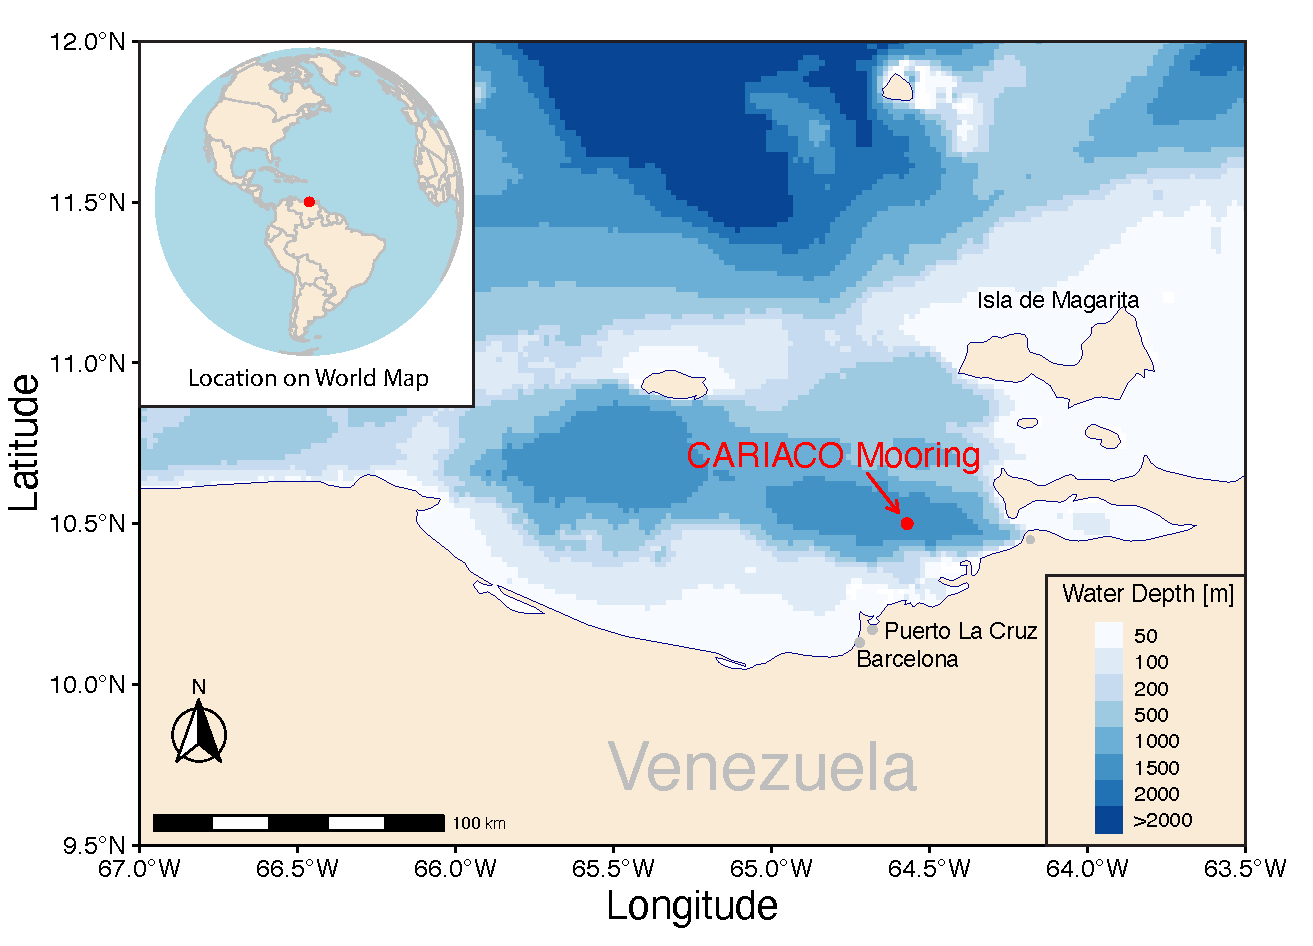
\includegraphics[width=\textwidth]{fig/Map_CAR.pdf}
\caption{Map of CARIACO Time Series location in the Cariaco basin in Venezuela in the Caribbean Ocean, located at \ang{10.50}N, \ang{64.67}W}
\label{fig:map}
\end{figure}

\begin{figure}
\noindent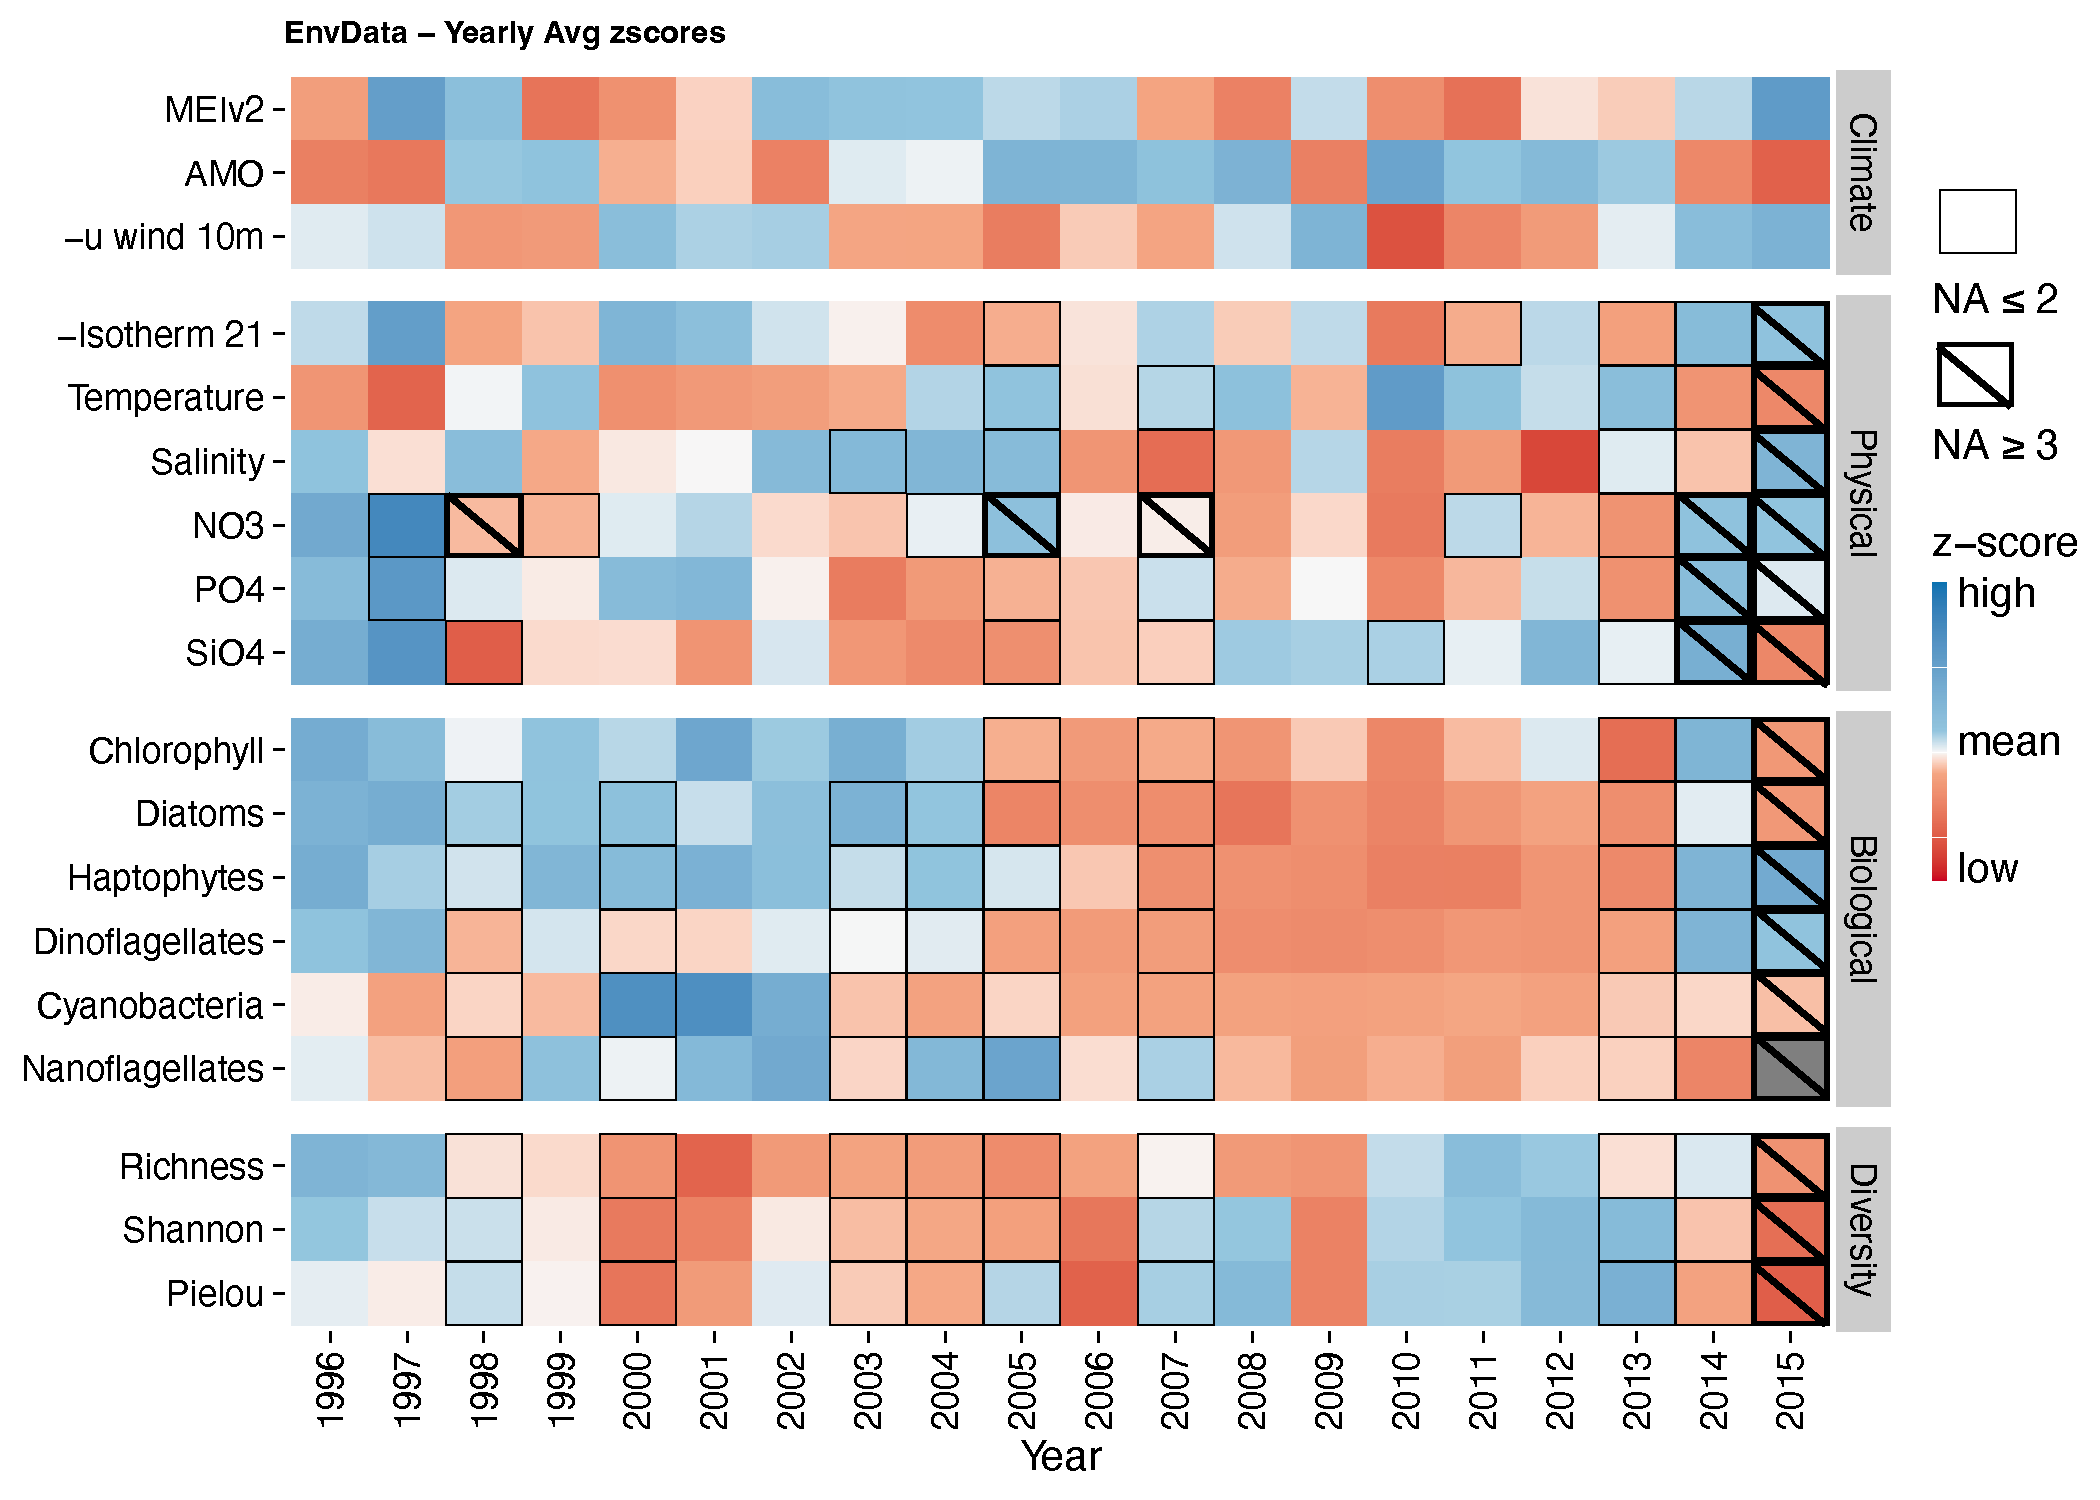
\includegraphics[width=\textwidth]{fig/PLOTZScores_updated.pdf}
\caption{Heatmap of yearly average values, normalized for comparison as z-scores. Red indicates a larger value, blue indicates a smaller value for that particular year. The years 1995 (n=2) and 2017 (n=1) were removed due to lack of data, additionally we marked years with two or less and three or more missing values. Diversity Indices are calculated based on microscopy counts at the Genus level.}
\label{fig:zscore}
\end{figure}

\begin{figure}
\begin{center}
\noindent\includegraphics[width=480pt]{fig/DepthDivTimeSeries_updated.pdf}
\end{center}
\caption{Time series and seasonality of chlorophyll \textit{a} and diversity indices across four depth intervals. (a,c,e,g) Annual mean across time series for years with more than 5 monthly sampling. Transparent dots show monthly raw values. (b,d,f,h) Boxplots of monthly measurements across four depth intervals grouped by season. Upwelling season lasts from December to April, Rainy Season from May to November.}
\label{fig:divts}
\end{figure}



\begin{figure}
\noindent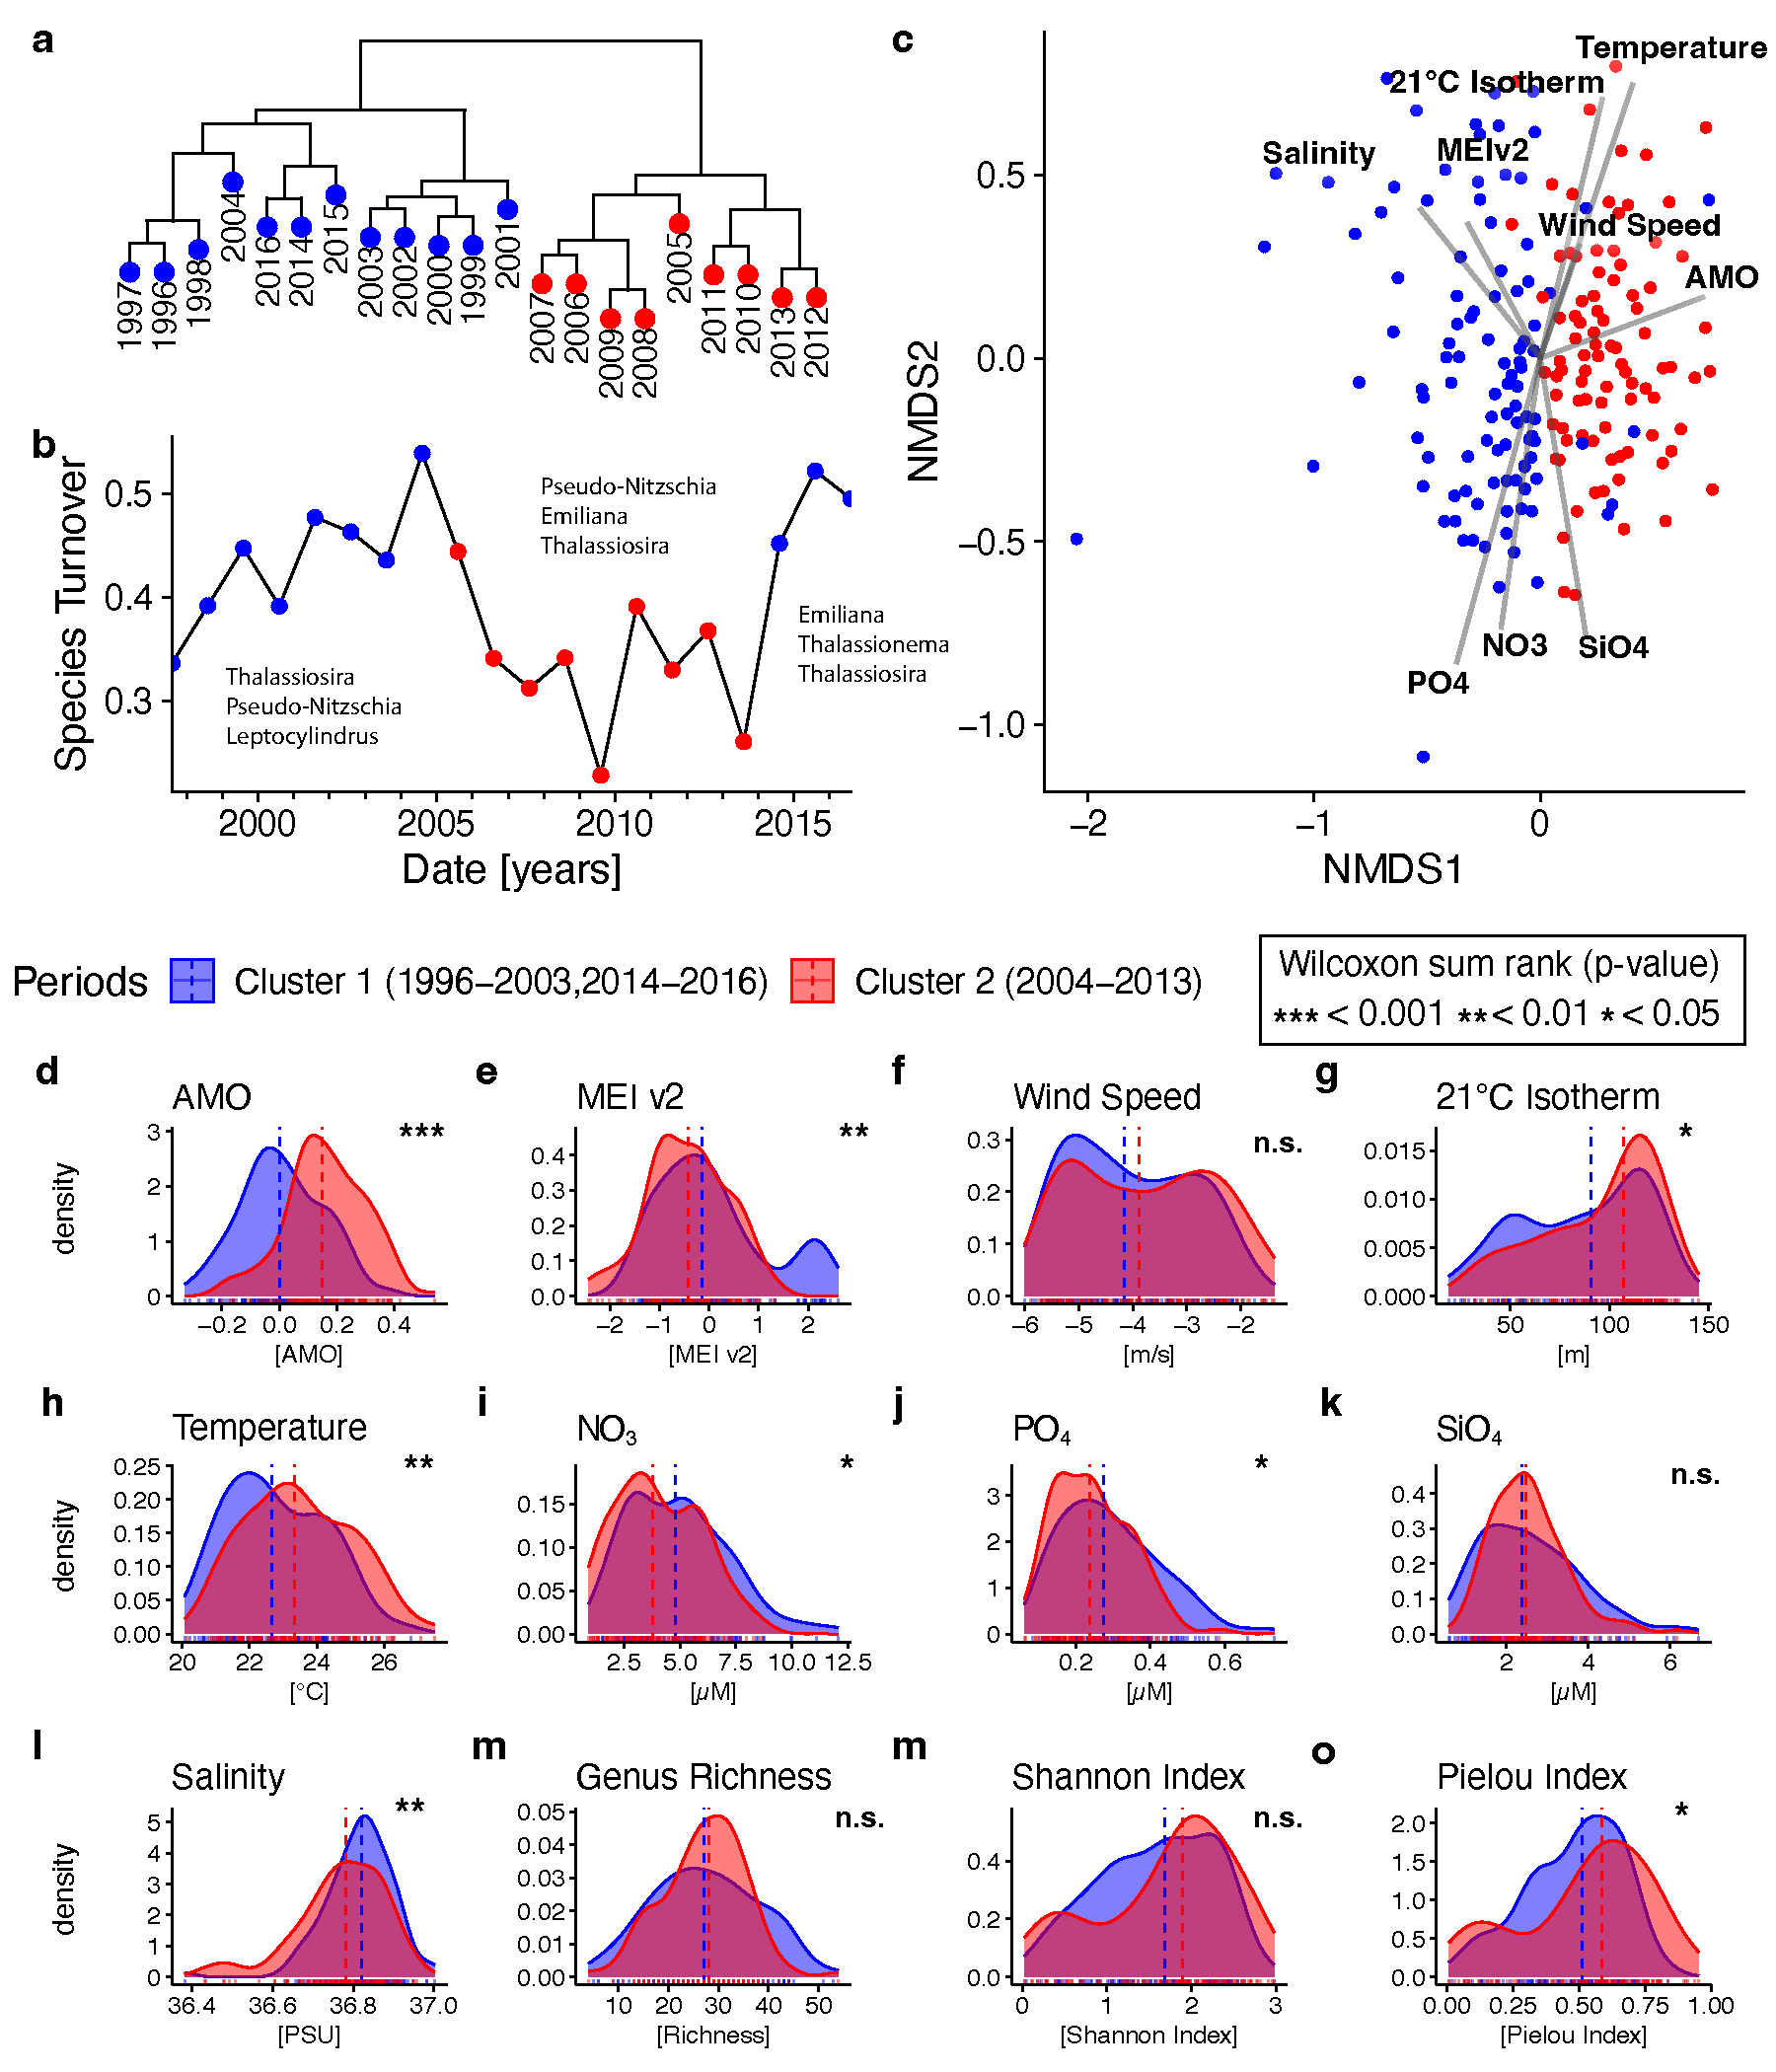
\includegraphics[width=\textwidth]{fig/ClusteringCompPlot_NEW 2.pdf}
\caption{(a) Clustering of microscopy data at the Genus level, using the binary Jaccard distance. The community for each year is binned together, to smooth out seasonal aspects. (b) Species turnover between years for annual aggregate of identified phytoplankton to a genus level. The three genera dominating the cell counts for the separate parts of cluster 1 and cluster 2 are given in order of abundance from top to bottom. (c) NMDS plot of monthly community data (cell counts) that is cube-root transformed. Stress: 0.261, 2 dimensions, converging solution. Color of dots based on which yearly cluster the monthly data is in. Vector overlay of ENVFIT shows underlying environmental variables that are co-varying with the community data.
Plots (d-o) below show density distributions of the environmental variables as well as diversity indices between the clustered years. Dashed line shows the median and significance levels of Wilcoxon sum rank tests between clusters are shown above plots  (***\textless0.001, **\textless0.01, *\textless0.05, n.s.=not significant).}
\label{fig:clustering}
\end{figure}

\begin{table}
\caption{Wilcoxon sum rank test with continuity correction for variables between the two clusters. Values for in-situ data are interpolated across the top 100 meters for each individual monthly cruise sampling.}
\label{table:clustering}
\centering
\begin{tabular}[t]{lrrl}
\toprule
Variable & W & p.value & Significance\\
\midrule
AMO & 3494.0 & 1.86e-14 & ***\\
MEI v.2 & 9523.5 & 0.006 & **\\
u-component 10 m wind speed & 7074.0 & 0.143 & n.s.\\
Isotherm \qty{21}{\celsius} & 5293.0 & 0.034 & *\\
\addlinespace
Temperature & 4763.0 & 0.003 & **\\
$NO_3$ & 6378.0 & 0.018 & *\\
$PO_4$ & 7359.0 & 0.012 & *\\
$SiO_4$ & 5998.0 & 0.736 & n.s.\\
Salinity & 7636.0 & 0.002 & **\\
\addlinespace
Genus Richness & 5913.0 & 0.954 & n.s.\\
Shannon Index & 5142.0 & 0.108 & n.s.\\
Pielou Index & 4874.0 & 0.029 & *\\
\bottomrule
\end{tabular}
\end{table}


\begin{figure}
\noindent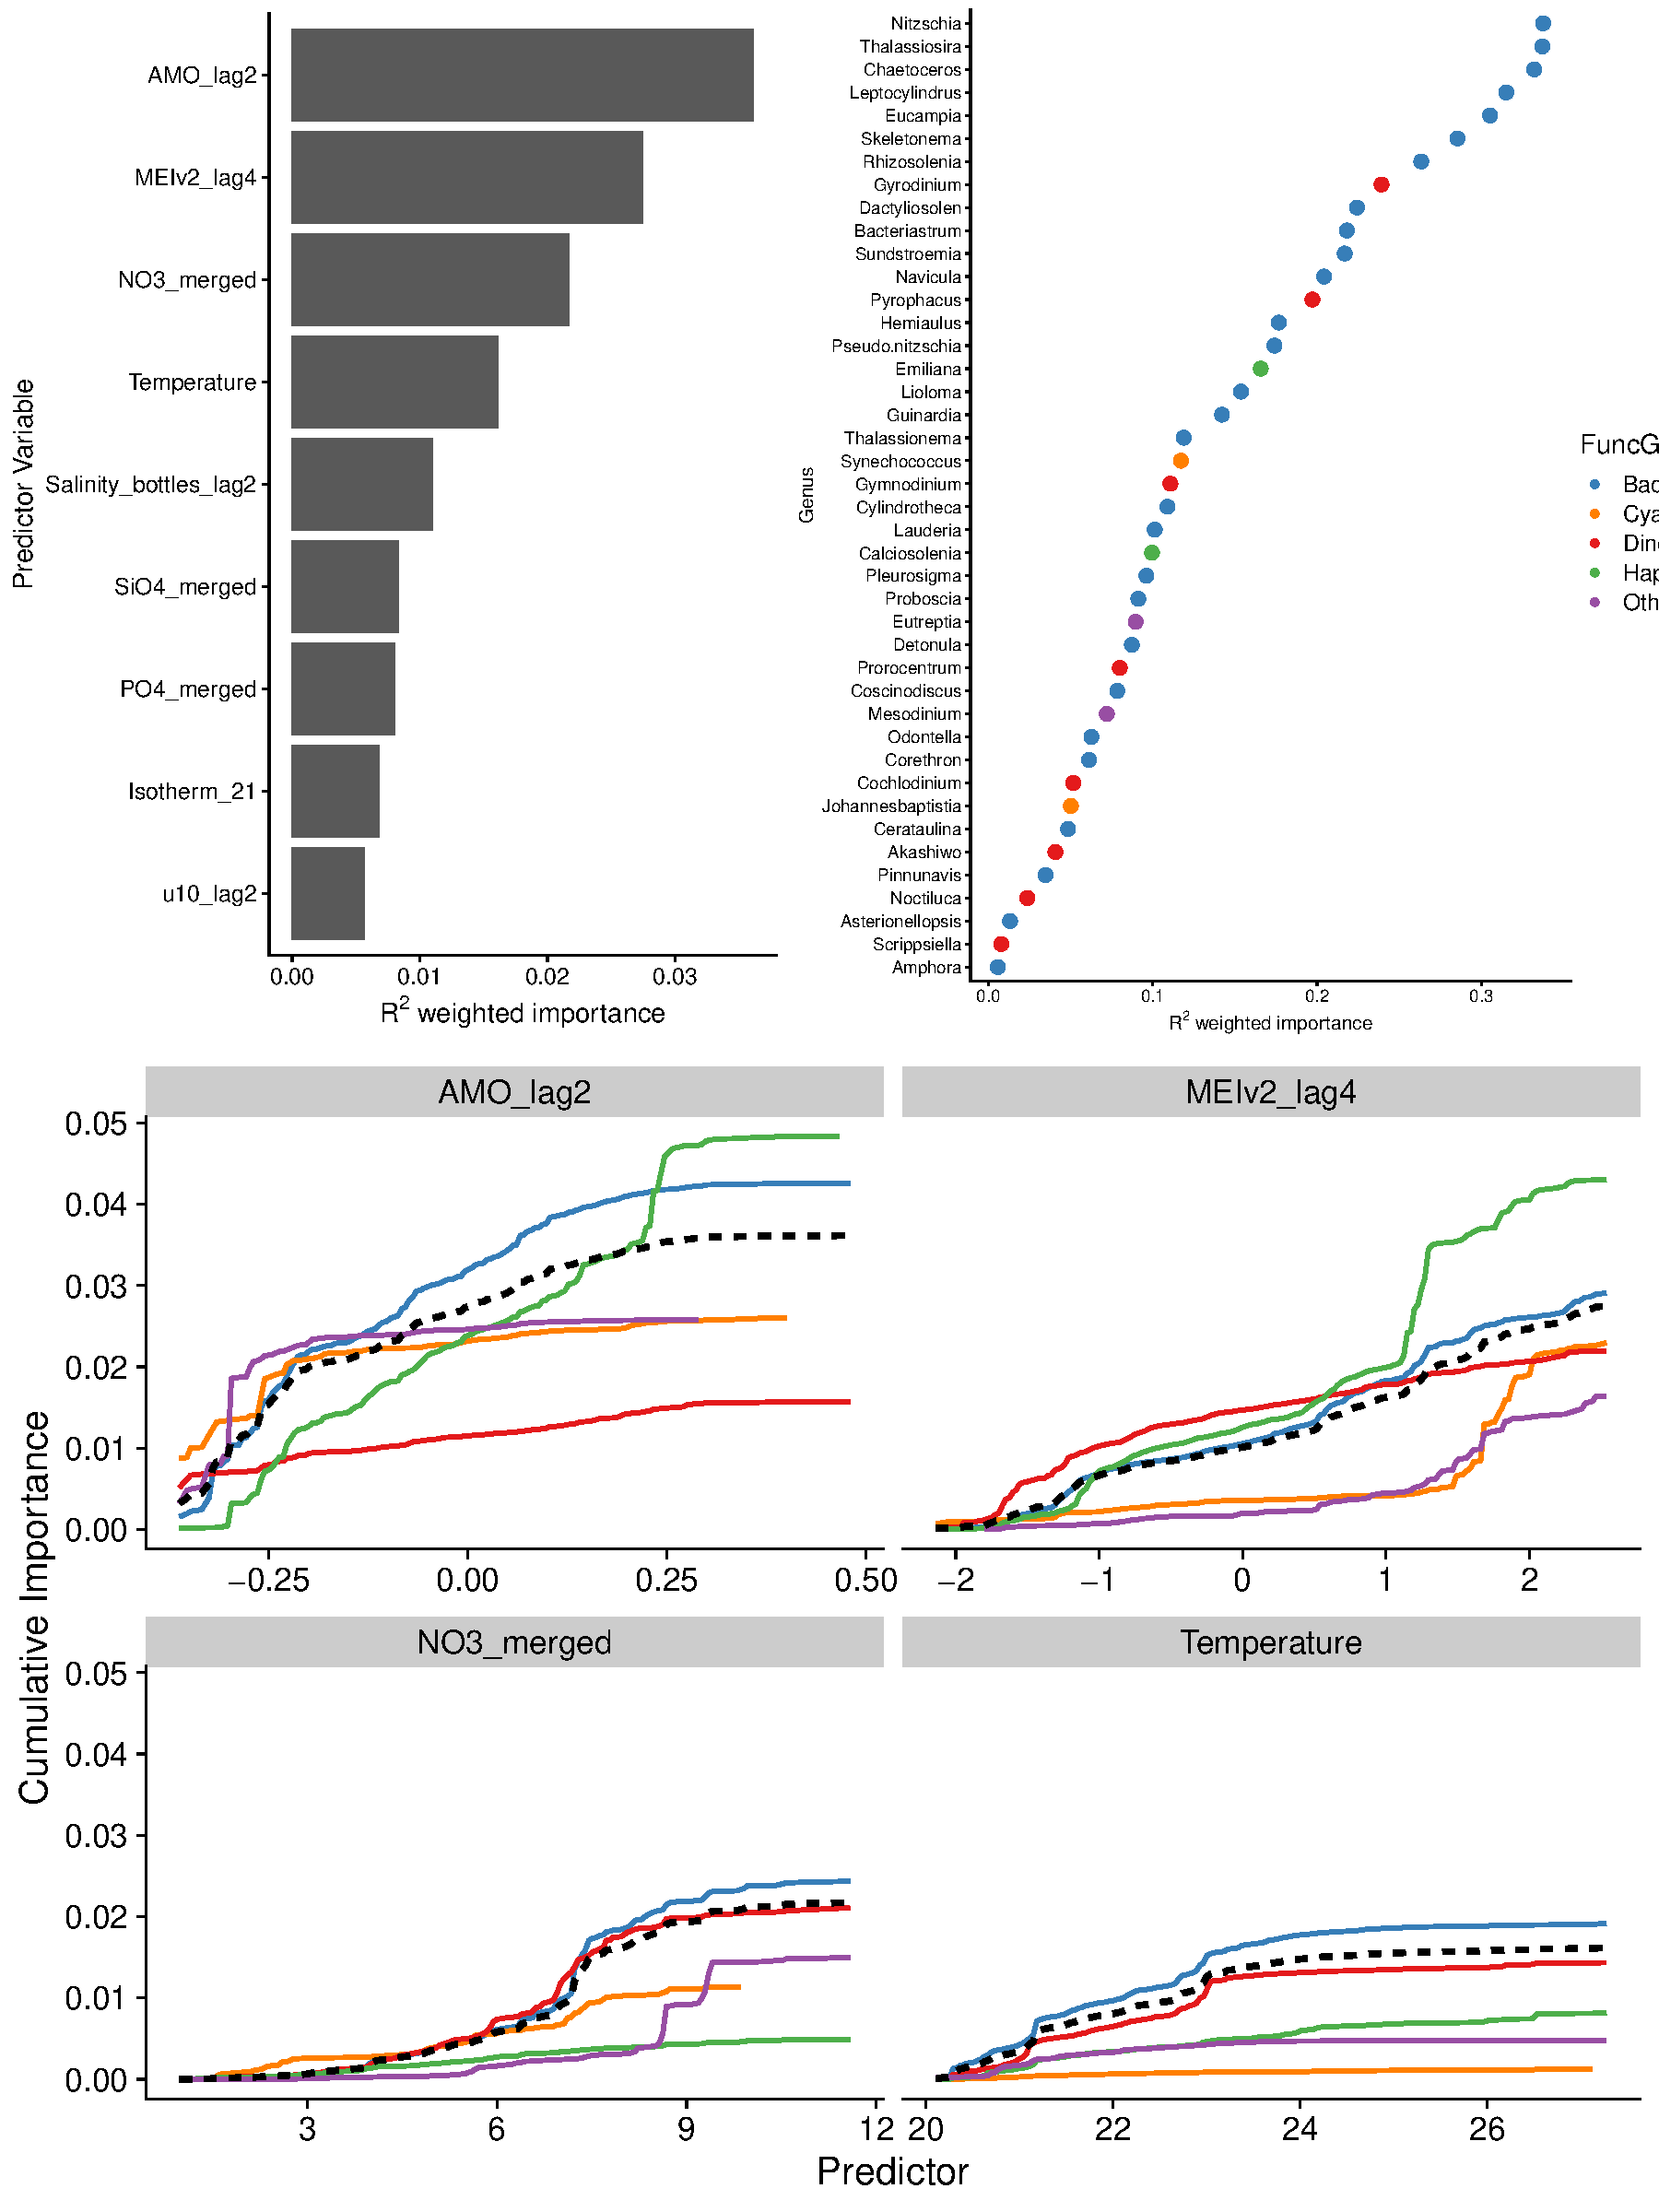
\includegraphics[width=\textwidth]{fig/GF_output_plot3_new.pdf}
\caption{Gradient Forest analysis of monthly community data at a genus level. (a) Predictor variables ranked according to overall weighted importance in predicting shifts in abundances. (b) Phytoplankton genera that could be predicted ranked according to the predictive power via the weighted importance. (c) Cumulative importance curves for the predictor variables. Black line shows cumulative importance across predictor range for the entire model and all genera. Dashed colored lines represent the responses of individual functional groups.}
\label{fig:GF}
\end{figure}


\section{Discussion}

This present study demonstrates the highly dynamic nature of a tropical coastal marine ecosystem driven by local environmental variability, which, in turn, is affected by large-scale climatic changes. In the Cariaco basin, decadal-scale climate oscillations have affected the wind-driven upwelling regime, which had confounding effects on the composition and biodiversity of the phytoplankton community.
% - a few sentences on basic seasonal dynamics removed here
These changes are well reflected in the yearly mean anomalies (see Figure \ref{fig:zscore}) and the density distribution of monthly measurements (see Figure \ref{fig:clustering}). After 2004 we see higher SST, lower wind speed, reduced fluorometric chlorophyll \textit{a}, a collapse in functional group cell counts, all matching a shift in the AMO toward positive mean anomalies until 2014. 
% - a few sentences about shift to smaller taxa and collapse in Sardine Fisheries

% - "We found that including the time series data until the end of 2017 in our analysis clearly shows that the observed shifts were reversible, confirming the observations by \citeA{muller-karger_scientific_2019}."
In 2014, physical conditions in the Cariaco basin returned to a regime of higher wind speeds, increased upwelling, and higher nutrient concentrations (see Figure \ref{fig:zscore}). At the same time, there was an increase in chlorophyll \textit{a} biomass (see Figure \ref{fig:divts} $a$) and a return to a community more similar to the period between 1996 and 2004 (see Figure \ref{fig:clustering} $a$ and $c$). This shift to a more productive phytoplankton community after 2014 also coincided with a recovery in sardine capture observed in 2016 and 2017 in a location south-east of the Isla de Magarita \cite{gomez_gaspar_variacion_2025}.

When comparing the phytoplankton community between the two clusters, we see a marked reduction in cell counts, which corresponds to a reduced concentration of chlorophyll \textit{a} biomass measured by fluorometry particularly in the top \qty{25}{meters} of the water column (see Figure \ref{fig:divts}). When including HPLC pigment data, these patterns are less clear, as the total chlorophyll measurement here actually shows an increase between the periods 1996-2000 and 2006-2010 \cite{pinckney_phytoplankton_2015}, particularly at depths below \qty{55}{meters}. It should be noted that the HPLC data were analyzed by multiple labs throughout the time series, with a gap in data coverage between 2000 and 2006. \citeA{pinckney_phytoplankton_2015} could not find a consistent method for quantifying total chlorophyll \textit{a} between the different laboratories. Here, we focus on the more consistently sampled fluorometric measurements. Independent spectophotometric measurements of chlorophyll \textit{a} concentration at \qty{20}{meters} depth off the coast of Magarita Island follow the temporal trend of a reduction in chlorophyll concentration between 2004 and 2014 \cite{gomez_gaspar_variacion_2025}. It should be noted that changes in the composition of the phytoplankton community can affect chlorophyll \textit{a} concentrations, as most measurement methods do not capture only chlorophyll \textit{a}, but also other related forms of chlorophyll, which can vary depending on the composition of the community \cite{welschmeyer_fluorometric_1994}.

Despite some of the difficulty in reconciling HPLC pigment data and microscopy cell counts, they agree in a reduction in diatom abundance after 2004. Cell counts of other functional groups decreased, where HPLC data indicate an increase and redistribution of biomass to depths below \qty{55}{meters} \cite{pinckney_phytoplankton_2015}. The decline in cell counts was not proportional to the more modest decrease in total chlorophyll \textit{a}, suggesting that the phytoplankton community transitioned to smaller individuals that were not captured under the microscope \cite{muller-karger_scientific_2019}. This shift to smaller cell sizes and a reduction in diatoms is consistent with predicted effects of warming and reduced mixing on phytoplankton communities \cite{bopp_response_2005}. Increases in temperature can lead to a decrease in the relative contribution of large cells in the community, irrespective of nutrient availability, but are particularly prevalent when (as observed in the Cariaco basin) temperatures increase and the nutrient supply decreases \cite{mousing_global_2014}. 

If we compare the two parts of the first cluster, the community did reorganize, particularly the diatoms shifted from a community dominated by centric diatoms (Guinardia, Leptocylindrus, Skeletonema) to one dominated by pennate diatoms (Pseudonitzschia) \cite{pinckney_phytoplankton_2015}.

However, the shift in yearly mean genus richness does not follow the abundances in the cell counts. Instead, we see a marked reduction following 1998 up until 2010, where richness recovers four years before the community seems to return to previous levels in 2014. The same trend is apparent, although to a less pronounced degree, in the other diversity metrics. Generally, mean anomalies in Shannon diversity and Pielou's evenness correlate with genus richness and show a reduced yearly mean between 2000 and 2006, during which time the cell counts registered an increase in nanoflagellates and a pronounced peak in cyanobacteria abundance. 

The period between 2001 and 2006 lacks coverage in HPLC data, so we have to rely on microscopy counts to deduce changes in the phytoplankton community. This limits the size range of the observable phytoplankton and the measurable diversity through the limited sampling volume \cite{cermeno_sampling_2014}. We can see a marked reduction in the genus richness of microphytoplankton ahead of the collapse in abundance, and similarly an increase a few years ahead of the return in abundance to previous levels. 
This pattern results in the fact that no significant differences in diversity are observed from microscopy cell counts between two clusters, either by Shannon index or by genus richness (see Figure \ref{fig:zscore} and \ref{fig:divts}).
We do see a significant difference in the Pilou index between the two clusters. Both HPLC pigment and microscopy measurements agree that the phytoplankton community became more evenly distributed during low-upwelling conditions of cluster 2 \cite{pinckney_phytoplankton_2015}. This increase in evenness, as quantified by Pilou's index, is most likely explained by the lack of strong upwelling events and the thereby reduced disturbance of the community. The resulting reduced compositional turnover is also observed in a decrease in interannual species turnover during cluster 2 (see Figure \ref{fig:clustering} $b$). As the productivity and biomass of phytoplankton communities are mainly driven by nutrients supplied through disturbance events, this confirms the previously observed inverse relationship between evenness and community performance \cite{lehtinen_phytoplankton_2017, otero_phytoplankton_2020}.

% NOW let's jump to Gradient Forest and discussing CLIMATE impacts! for a final paragraph, and then we are done here!!
To identify the variables that can best predict changes in the phytoplankton community, we used a gradient forest analysis using microscopy cell counts at the genus level as predicted variables and climate indices and in situ measurements of bottom-up drivers as predictors. Limiting the analysis to bottom-up drivers ensured the greatest possible data coverage throughout the CARIACO time series. Interestingly, our analysis found that the strongest predictors of changes within the community are not in situ measurements, but actually the AMO and the MEI v.2 climate indices. These are followed in importance by nitrate concentration and temperature in the upper \qty{100}{meters} (see Figure \ref{fig:GF}).

These results match the observed NMDS clustering of the monthly cell counts in relation to the predictor variables, since the scaling axis that separates the two yearly aggregate community clusters is NMDS 1, which covaries most strongly with changes in the AMO, MEI v.2 (see Figure \ref{fig:clustering} $c$). Variables directly related to upwelling conditions, such as temperature, \qty{21}{\celsius} isotherm, wind speed, and nutrient concentrations vary more strongly along NMDS2. This indicates that the climate indices capture some variability, which is not represented in the more direct measurements of upwelling intensity. Salinity and silicate concentration, which are also strongly related to water mass exchanges through upwelling, but also depend on precipitation and fresh water input through surface runoff, show greater variance along NMDS1. Both salinity and silicate concentration show some explanatory power in the gradient forest analysis, although they are weaker predictors than temperature, nitrate concentration, and the climate indices. 

Using microscopy cell counts as a basis for this analysis meant that the results should be interpreted in terms of changes in the microphytoplankton community, due to the size limitation of identifying smaller species via light microscopy. Grouping cell counts by genera does create a loss of resolution, but is based on the assumption that species within a genus generally show similar ecophysiological responses. The output of the gradient forest model is further grouped by broad functional types to facilitate the identification of shifts and trends. The phytoplankton genera that can be best predicted are mostly diatoms, but also some haptophytes, dinoflagellates, and cyanobacteria (see Figure \ref{fig:GF} $b$). Within these groups, we see differing threshold responses in cumulative importance along the predictor ranges.

AMO has emerged as an important indicator of the climate system and how it affects the ecosystems of the north Atlantic \cite{nye_ecosystem_2014}. The oscillations of the AMO index are strongly correlated with temperature indices in the Caribbean region \cite{stephenson_changes_2014}. Although regional effecs may vary, a positive phase in the AMO is generally associated with periods of warmer temperatures and a shift of the ITCZ from north to south. This shift of the ITCZ southward increases wind-driven upwelling in the Cariaco basin \cite{taylor_ecosystem_2012}. The threshold responses between functional groups, which relate to a shift in the cell count abundances, show contrasting patterns. Diatoms and cyanobacteria show strong response thresholds for negative AMO anomalies. This is an interesting threshold response shown for the AMO, which, if sufficiently negative, seems to correlate to a reorganization of the physical regime in the Cariaco basin. The abundance of haptophytes shows a strong threshold at positive AMO anomalies, which could be related to the pattern observed from HPLC data of haptophytes mostly exhibiting blooms above the mixed layer and at a lower frequency from other functional groups \cite{pinckney_phytoplankton_2015}.

% Move the general point on ENSO to intro! Only Discussion-relevant part here..
The El Niño Southern Osciallation (ENSO) has a strong teleconnection to the Caribbean Sea, since during ENSO (indicated by a positive MEI v.2 index) sea surface temperatures rise and trade winds blow more to the north-northwest \cite{enfield_tropical_1997}. \citeA{taylor_ecosystem_2012} found no strong correlation between the MEI v.2 and measuerments in the Cariaco basin, and only \qtyrange{24}{36}{\%} explanantion of variance with a time lag of 12 months using linear regression. In contrast, we found a relatively strong predictive power for changes in the phytoplankton community with a 4-month time lag. We also tested a 12 month lag and found no significant improvement.
The threshold responses show a shift in the abundances of dinoflagellates and haptophytes for a negative MEI v.2 index, which indicates La Niña conditions. For cyanobacteria and haptophytes, we found a pronounced threshold response for positive anomalies showing a sensitivity to ENSO events. Diatoms do not show a clear threshold response for the MEI v.2 index, but are affected across the entire range. Positive anomalies of the MEI v.2, representing strong ENSO events, are interestingly only found in Cluster 1 (see Figure \ref{fig:clustering} $e$). 

The in-situ measurements that best predict changes in the microphytoplankton community were nitrate concentration, temperature and salinity, in that order. Nitrate is a central nutrient for phytoplankton growth and has been found to be the growth-limiting nutrient during stratification periods in the Cariaco basin \cite{muller-karger_scientific_2019}. For dinoflagellates and diatoms, we see a strong threshold response around \qty{7}{\micro \mole}, which would indicate that strong upwelling conditions drive blooms of these functional groups. Other functional groups including \textit{Mesodinium} and \textit{Eutreptria} also show a threshold response at even higher nitrate concentrations (around \qty{9}{\micro \mole}), indicating an effect on their abundance by very strong upwelling. Similarly, for temperature, dinoflagellates and diatoms show a threshold around \qtyrange{21}{23}{\celsius}, which indicates higher abundances during low temperatures in the upper \qty{100}{m} driven by strong upwelling. For the other predictors, we do not see strong threshold responses.

Gradient forest analysis clearly identified the AMO and MEI v.2 climate indices as the best predictors of changes in the microphytoplankton community in the Cariaco basin. This is an interesting result, as it would be expected that more direct measures of ecosystem variability could better predict shifts in abundances. One possible explanation is that in situ measurements contain much stronger variability due to measurement error, local and temporal variability, and generally only provide a single snapshot for an entire month. Climate indices are detrended and integrated measurements of long-term changes that are matching in scale to the dynamics of long-term changes within a phytoplankton community. However, we do not see such strong predictive power in the ERA5 climate reanalysis-derived mean wind speed, which also aggregates measurements and model output over an entire month. 
Another explanation could be that the climate indices capture a dimension of variability not found in our in-situ measurements, which is also represented in our NMDS clustering (see Figure \ref{fig:clustering} $c$), where both MEI v.2 and AMO scale along the second axis (NMDS 2). %TODO test more of my variables along these axes, then add to discussion here and maybe put plot in supplemental material.

% FROM FRAKER ET AL. 2022
%"Note that although this analysis identifies predictive relationships between drivers and the biological indicators, these relationships do not necessarily imply mechanistic relationships. As such, this analysis represents the first stages of an overall analysis (a narrowing of the potential key relationships and when they matter from a much larger dataset), and additional statistical analyses, modeling, and experimental work may be required to develop a full mechanistic understanding of driver-response relationships and ecosystem change."

Our limitation to bottom-up drivers of community change could also limit the explanatory power of our analysis, as top-down processes such as zooplankton grazing strongly affect the structure of the phytoplankton community \cite{banas_adding_2011, acevedo-trejos_mechanisms_2015}. In the Cariaco basin in particular, a trophic cascade from the collapse of sardine fisheries through an increasing abundance of mesozooplaknton has been proposed to have affected the phytoplankton community \cite{muller-karger_scientific_2019}. Due to the lack of temporal resolution for higher trophic levels and the lack of zooplankton data for the first 6 years of the time series, we propose that mechanistic modeling studies could be well suited to investigate this aspect of the CARIACO time series further.

In this study, we have found a strong impact of decadal-scale climatic oscillations on shifts in the phytoplankton community in the tropical coastal ecosystem of the Cariaco basin. Despite multiannual trends in warming, reduced productivity and a collapse in fisheries and phytoplankton cell counts, the phytoplankton community returned to previous levels once the climatic and local physical conditions returned. We see these patterns clearly in the community data retrieved from microscopy, which shows the value of the arduous work of identifying and counting phytoplankton cells. The strongest bottom-up variable predicting changes in the phytoplankton community is the AMO index, highlighting the complex nature of climate-driven ecosystem variability and the connections between global climate and local ecosystems through low-frequency natural cycles. We hope that the work hints at the resilient nature of phytoplankton communities under global change, which should be further investigated by studying long-term ocean time series.

% Highlight that the climate indices explain changes in the community and abundance, but not necessarily changed in diversity (as there is no sig diff beteween clusters). Probably need more data, other approaches to untangle effects on diversity.





\section{Conclusions}
% Theoretically the final paragraph above represents the conclusion

- Our analysis shows that...

- We also show that...

- But we cannot confirm or test. so we would recommend X for the future.






%%

%  Numbered lines in equations:
%  To add line numbers to lines in equations,
%  \begin{linenomath*}
%  \begin{equation}
%  \end{equation}
%  \end{linenomath*}



%% Enter Figures and Tables near as possible to where they are first mentioned:
%
% DO NOT USE \psfrag or \subfigure commands.
%
% Figure captions go below the figure.
% Acronyms used in figure captions will be spelled out in the final, published version.

% Table titles go above tables;  other caption information
%  should be placed in last line of the table, using
% \multicolumn2l{$^a$ This is a table note.}
% NOTE that there is no difference between table caption and table heading in the final, published version
%
%----------------
% EXAMPLE FIGURES
%
% \begin{figure}
% \includegraphics{example.png}
% \caption{caption}
% \end{figure}
%
% Giving latex a width will help it to scale the figure properly. A simple trick is to use \textwidth. Try this if large figures run off the side of the page.
% \begin{figure}
% \noindent\includegraphics[width=\textwidth]{anothersample.png}
%\caption{caption}
%\label{pngfiguresample}
%\end{figure}
%
%
% If you get an error about an unknown bounding box, try specifying the width and height of the figure with the natwidth and natheight options. This is common when trying to add a PDF figure without pdflatex.
% \begin{figure}
% \noindent\includegraphics[natwidth=800px,natheight=600px]{samplefigure.pdf}
%\caption{caption}
%\label{pdffiguresample}
%\end{figure}
%
%
% PDFLatex does not seem to be able to process EPS figures. You may want to try the epstopdf package.
%

%
% ---------------
% EXAMPLE TABLE
%
% \begin{table}
% \caption{Time of the Transition Between Phase 1 and Phase 2$^{a}$}
% \centering
% \begin{tabular}{l c}
% \hline
%  Run  & Time (min)  \\
% \hline
%   $l1$  & 260   \\
%   $l2$  & 300   \\
%   $l3$  & 340   \\
%   $h1$  & 270   \\
%   $h2$  & 250   \\
%   $h3$  & 380   \\
%   $r1$  & 370   \\
%   $r2$  & 390   \\
% \hline
% \multicolumn{2}{l}{$^{a}$Footnote text here.}
% \end{tabular}
% \end{table}

%%%%%%%%%%%%%%%%%%%%%%%%%%%%%%%%%%%%%%%%%%%%%%%
% SIDEWAYS FIGURES and TABLES
% AGU prefers the use of {sidewaystable} over {landscapetable} as it causes fewer problems.
%
% \begin{sidewaysfigure}
% \includegraphics[width=20pc]{figsamp}
% \caption{caption here}
% \label{newfig}
% \end{sidewaysfigure}
%
%  \begin{sidewaystable}
%  \caption{Caption here}
% \label{tab:signif_gap_clos}
%  \begin{tabular}{ccc}
% one&two&three\\
% four&five&six
%  \end{tabular}
%  \end{sidewaystable}

%% If using numbered lines, please surround equations with \begin{linenomath*}...\end{linenomath*}
%\begin{linenomath*}
%\begin{equation}
%y|{f} \sim g(m, \sigma),
%\end{equation}
%\end{linenomath*}

%%% End of body of article

%%%%%%%%%%%%%%%%%%%%%%%%%%%%%%%%%%%%%%%%%%%%%%%
%% Optional Appendices go here
%
% The \appendix command resets counters and redefines section heads
%
% After typing \appendix
%
%\section{Here Is Appendix Title}
% will show
% A: Here Is Appendix Title
%

\appendix

\section{Gradient Forest Analysis supplement}


\begin{table}

\caption{Individual Gradient Forest model runs for each variable and the corresponding time lags. 
        For in-situ variables, for which no coverage extends over the time series, 
        we tested all measurements up to a lag of 3 months. 
        For climate variables, we tested up to a lag of 6 months. 
        Time lag with maximum importance per variable are highlighted in bold and chosen for the final model run.}
        
\ref{app:table1}
\centering
\begin{tabular}[t]{rrrrrrrrrr}
\toprule
lag & NO3 & PO4 & SiO4 & Temperature & Isotherm\_21 & Salinity\_bottles & u10 & AMO & MEIv2\\
\midrule
0 & \textbf{0.038} & \textbf{0.038} & \textbf{0.034} & \textbf{0.071} & \textbf{0.028} & 0.007 & 0.004 & 0.016 & 0.015\\
1 & 0.017 & 0.011 & 0.015 & 0.002 & 0.002 & 0.004 & \textbf{0.010} & 0.014 & 0.018\\
2 & 0.022 & 0.008 & 0.013 & 0.006 & 0.008 & \textbf{0.011} & 0.009 & \textbf{0.030} & 0.019\\
3 & 0.016 & 0.007 & 0.004 & 0.005 & 0.007 & 0.010 & 0.007 & 0.018 & 0.018\\
4 & - & - & - & - & - & - & 0.008 & 0.019 & \textbf{0.029}\\
5 & - & - & - & - & - & - & 0.008 & 0.018 & 0.022\\
6 & - & - & - & - & - & - & 0.010 & 0.018 & 0.013\\
\bottomrule
\end{tabular}
\end{table}


%%%%%%%%%%%%%%%%%%%%%%%%%%%%%%%%%%%%%%%%%%%%%%%
% Optional Glossary, Notation or Acronym section goes here:
%
% Glossary is only allowed in Reviews of Geophysics
%  \begin{glossary}
%  \term{Term}
%   Term Definition here
%  \term{Term}
%   Term Definition here
%  \term{Term}
%   Term Definition here
%  \end{glossary}


%%%%%%%%%%%%%%%%%%%%%%%%%%%%%%%%%%%%%%%%%%%%%%%
% Acronyms
%% NOTE that acronyms in the final published version will be spelled out when used in figure captions.
%   \begin{acronyms}
%   \acro{Acronym}
%   Definition here
%   \acro{EMOS}
%   Ensemble model output statistics
%   \acro{ECMWF}
%   Centre for Medium-Range Weather Forecasts
%   \end{acronyms}


%%%%%%%%%%%%%%%%%%%%%%%%%%%%%%%%%%%%%%%%%%%%%%%
% Notation
%   \begin{notation}
%   \notation{$a+b$} Notation Definition here
%   \notation{$e=mc^2$}
%   Equation in German-born physicist Albert Einstein's theory of special
%  relativity that showed that the increased relativistic mass ($m$) of a
%  body comes from the energy of motion of the body—that is, its kinetic
%  energy ($E$)—divided by the speed of light squared ($c^2$).
%   \end{notation}




%%%%%%%%%%%%%%%%%%%%%%%%%%%%%%%%%%%%%%%%%%%%%%%
%
% DATA SECTION and ACKNOWLEDGMENTS
%
%%%%%%%%%%%%%%%%%%%%%%%%%%%%%%%%%%%%%%%%%%%%%%%

%!
\section*{Open Research Section}
This section MUST contain a statement that describes where the data supporting the conclusions can be obtained. Data cannot be listed as ''Available from authors'' or stored solely in supporting information. Citations to archived data should be included in your reference list. Wiley will publish it as a separate section on the paper’s page. Examples and complete information are here:
https://www.agu.org/Publish with AGU/Publish/Author Resources/Data for Authors

\section*{As Applicable – Inclusion in Global Research Statement}
The Authorship: Inclusion in Global Research policy aims to promote greater equity and transparency in research collaborations. AGU Publications encourage research collaborations between regions, countries, and communities and expect authors to include their local collaborators as co-authors when they meet the AGU Publications authorship criteria (described here: https://www.agu.org/publications/authors/policies\#authorship). Those who do not meet the criteria should be included in the Acknowledgement section. We encourage researchers to consider recommendations from The TRUST CODE - A Global Code of Conduct for Equitable Research Partnerships (https://www.globalcodeofconduct.org/) when conducting and reporting their research, as applicable, and encourage authors to include a disclosure statement pertaining to the ethical and scientific considerations of their research collaborations in an “Inclusion in Global Research Statement’ as a standalone section in the manuscript following the Conclusions section. This can include disclosure of permits, authorizations, permissions and/or any formal agreements with local communities or other authorities, additional acknowledgements of local help received, and/or description of end-users of the research. You can learn more about the policy in this editorial. Example statements can be found in the following published papers: 
%Holt et al. (https://agupubs.onlinelibrary.wiley.com/doi/full/10.1029/2022JG007188), 
%Sánchez-Gutiérrez et al. (https://agupubs.onlinelibrary.wiley.com/doi/abs/10.1029/2023JG007554), 
%Tully et al. (https://agupubs.onlinelibrary.wiley.com/doi/epdf/10.1029/2022JG007128) 
%Please note that these statements are titled as “Global Research Collaboration Statements” from a previous pilot requirement in JGR Biogeosciences. The pilot has ended and statements should now be titled “Inclusion in Global Research Statement”.


%!
\acknowledgments
Thank you to all who have helped, communicated, provided data. Claudia Benitez-Nelson, Digna Rueda-Roa, James Pinckney.

%Enter acknowledgments here. This section is to acknowledge funding, thank colleagues, enter any secondary affiliations, and so on.


%%%%%%%%%%%%%%%%%%%%%%%%%%%%%%%%%%%%%%%%%%%%%%%
% REFERENCES and BIBLIOGRAPHY
%
%\bibliography{<name of your .bib file>} don't specify the file extension
% don't specify bibliographystyle
%
%%%%%%%%%%%%%%%%%%%%%%%%%%%%%%%%%%%%%%%%%%%%%%%

\bibliography{references}



%Reference citation instructions and examples:
%
% Please use ONLY \cite and \citeA for reference citations.
% \cite for parenthetical references
% ...as shown in recent studies (Simpson et al., 2019)
% \citeA for in-text citations
% ...Simpson et al. (2019) have shown...
%
%
%...as shown by \citeA{jskilby}.
%...as shown by \citeA{lewin76}, \citeA{carson86}, \citeA{bartoldy02}, and \citeA{rinaldi03}.
%...has been shown \cite{jskilbye}.
%...has been shown \cite{lewin76,carson86,bartoldy02,rinaldi03}.
%... \cite <i.e.>[]{lewin76,carson86,bartoldy02,rinaldi03}.
%...has been shown by \cite <e.g.,>[and others]{lewin76}.
%
% apacite uses < > for prenotes and [ ] for postnotes
% DO NOT use other cite commands (e.g., \citet, \citep, \citeyear, \nocite, \citealp, etc.).
%




\end{document}



More Information and Advice:

%%%%%%%%%%%%%%%%%%%%%%%%%%%%%%%%%%%%%%%%%%%%%%%
%
%  SECTION HEADS
%
%%%%%%%%%%%%%%%%%%%%%%%%%%%%%%%%%%%%%%%%%%%%%%%

% Capitalize the first letter of each word (except for
% prepositions, conjunctions, and articles that are
% three or fewer letters).

% AGU follows standard outline style; therefore, there cannot be a section 1 without
% a section 2, or a section 2.3.1 without a section 2.3.2.
% Please make sure your section numbers are balanced.
% ---------------
% Level 1 head
%
% Use the \section{} command to identify level 1 heads;
% type the appropriate head wording between the curly
% brackets, as shown below.
%
%An example:
%\section{Level 1 Head: Introduction}
%
% ---------------
% Level 2 head
%
% Use the \subsection{} command to identify level 2 heads.
%An example:
%\subsection{Level 2 Head}
%
% ---------------
% Level 3 head
%
% Use the \subsubsection{} command to identify level 3 heads
%An example:
%\subsubsection{Level 3 Head}
%
%---------------
% Level 4 head
%
% Use the \subsubsubsection{} command to identify level 3 heads
% An example:
%\subsubsubsection{Level 4 Head} An example.
%
%%%%%%%%%%%%%%%%%%%%%%%%%%%%%%%%%%%%%%%%%%%%%%%
%
%  IN-TEXT LISTS
%
%%%%%%%%%%%%%%%%%%%%%%%%%%%%%%%%%%%%%%%%%%%%%%%
%
% Do not use bulleted lists; enumerated lists are okay.
% \begin{enumerate}
% \item
% \item
% \item
% \end{enumerate}
%
%%%%%%%%%%%%%%%%%%%%%%%%%%%%%%%%%%%%%%%%%%%%%%%
%
%  EQUATIONS
%
%%%%%%%%%%%%%%%%%%%%%%%%%%%%%%%%%%%%%%%%%%%%%%%

% Single-line equations are centered.
% Equation arrays will appear left-aligned.

Math coded inside display math mode \[ ...\]
 will not be numbered, e.g.,:
 \[ x^2=y^2 + z^2\]

 Math coded inside \begin{equation} and \end{equation} will
 be automatically numbered, e.g.,:
 \begin{equation}
 x^2=y^2 + z^2
 \end{equation}


% To create multiline equations, use the
% \begin{eqnarray} and \end{eqnarray} environment
% as demonstrated below.
\begin{eqnarray}
  x_{1} & = & (x - x_{0}) \cos \Theta \nonumber \\
        && + (y - y_{0}) \sin \Theta  \nonumber \\
  y_{1} & = & -(x - x_{0}) \sin \Theta \nonumber \\
        && + (y - y_{0}) \cos \Theta.
\end{eqnarray}

%If you don't want an equation number, use the star form:
%\begin{eqnarray*}...\end{eqnarray*}

% Break each line at a sign of operation
% (+, -, etc.) if possible, with the sign of operation
% on the new line.

% Indent second and subsequent lines to align with
% the first character following the equal sign on the
% first line.

% Use an \hspace{} command to insert horizontal space
% into your equation if necessary. Place an appropriate
% unit of measure between the curly braces, e.g.
% \hspace{1in}; you may have to experiment to achieve
% the correct amount of space.


%%%%%%%%%%%%%%%%%%%%%%%%%%%%%%%%%%%%%%%%%%%%%%%
%
%  EQUATION NUMBERING: COUNTER
%
%%%%%%%%%%%%%%%%%%%%%%%%%%%%%%%%%%%%%%%%%%%%%%%

% You may change equation numbering by resetting
% the equation counter or by explicitly numbering
% an equation.

% To explicitly number an equation, type \eqnum{}
% (with the desired number between the brackets)
% after the \begin{equation} or \begin{eqnarray}
% command.  The \eqnum{} command will affect only
% the equation it appears with; LaTeX will number
% any equations appearing later in the manuscript
% according to the equation counter.
%

% If you have a multiline equation that needs only
% one equation number, use a \nonumber command in
% front of the double backslashes (\\) as shown in
% the multiline equation above.

% If you are using line numbers, remember to surround
% equations with \begin{linenomath*}...\end{linenomath*}

%  To add line numbers to lines in equations:
%  \begin{linenomath*}
%  \begin{equation}
%  \end{equation}
%  \end{linenomath*}



